\documentclass[11pt]{article}
\usepackage[a4paper,margin=2.3cm]{geometry}
\usepackage{amsmath,amssymb,amsthm}
\usepackage{graphicx}
\usepackage{booktabs}
\usepackage{longtable}
\usepackage{array}
\usepackage{caption}
\usepackage{float}
\usepackage[hidelinks]{hyperref}
\usepackage{xcolor}
\usepackage{enumitem}
\setlength{\parskip}{3pt}
\captionsetup{font=small,labelfont=bf}
\newtheorem{definition}{Definition}[section]
\newtheorem{proposition}[definition]{Proposition}
\newtheorem{theorem}[definition]{Theorem}
\newtheorem{lemma}[definition]{Lemma}
\newtheorem{remark}[definition]{Remark}
\newtheorem{conjecture}[definition]{Conjecture}
\newcommand{\R}{\mathbb{R}}
\newcommand{\N}{\mathcal{N}}
\newcommand{\U}{\mathcal{U}}
\newcommand{\D}{\mathbb{D}}
\newcommand{\Lie}{\mathcal{L}}
\newcommand{\cat}[1]{\mathbf{#1}}
\newcommand{\nSystems}{52}
\newcommand{\nAtom}{16}
\newcommand{\nBackbone}{36}
\newcommand{\nPaired}{35}
\newcommand{\nMdcath}{35}
\newcommand{\sepRatio}{1.70}
\newcommand{\sepP}{0.000}


\title{Fluid nerve theory: deformation fields, ambient-time filtrations and\\synthetic differential geometry for a molecular atlas of \nSystems{} systems}
\author{Joseph Campagna, PSM\\[2pt]\small with the pronerv fluid-nerve pipeline (code and data provenance in the repository)}
\date{\today}

\begin{document}
\maketitle

\begin{abstract}
The pronerv molecular atlas drew categorical overlap nerves for two systems, alanine dipeptide (heavy atoms) and chignolin CLN025 (C$\alpha$ sites). This document extends the construction to \nSystems{} systems, half atom-based and half backbone-based (\nAtom{} heavy-atom systems, \nBackbone{} C$\alpha$ systems, plus \nPaired{} paired heavy-atom representations of the backbone proteins), builds for each a \emph{deformation field} and a \emph{witnessed cover nerve}, runs an \emph{ambient-time filtration} that thickens the cover along the recorded dynamics, and compares the resulting invariants within and between the two groups. Every nerve is also exported as a three-dimensional categorical complex for the proof assistant homotopy.io through Street's orientals. The theoretical part recruits synthetic differential geometry (Kock--Lawvere) to say precisely what a deformation field is at an infinitesimal scale, proves that the nerve of a formally open cover is rigid under every infinitesimal transformation, and hence identifies the measured ambient-time persistence as a finite-time, finite-witness phenomenon whose onset is diagnosed by the mobility exponent. The empirical constructions are descriptive: no equilibrium free energy, validated kinetics or configuration-space nerve theorem is claimed.
\end{abstract}

\tableofcontents

\section{Why ``fluid'' nerves}
A nerve is a static object: given a cover $\U=\{U_i\}$ of a space, its simplices record which cover sets meet. Molecular dynamics (MD) data are not static. A recorded trajectory visits the chart, and the overlap pattern that a finite set of frames \emph{witnesses} changes with the time scale at which we look. The earlier atlas treated this by declaring a single cover and a single lag for the structural-mobility height. Here we make the time dependence explicit in two ways:
\begin{enumerate}[nosep]
\item the \textbf{deformation field}, a family of conditional statistics of the lag-$\tau$ displacement, indexed by the chart position and by the ambient lag $\tau$;
\item the \textbf{fluid filtration}, the nested family of nerves of the covers $\{W_i^{\tau}\}$ obtained by thickening every cover set along the recorded runs by $\pm\tau$ frames.
\end{enumerate}
``Fluid nerve'' names the pair (nerve, deformation field) together with its evolution in ambient time. The synthetic differential geometry (SDG) of Section~\ref{sec:sdg} explains what survives of this evolution at an infinitesimal scale, which is less than one might hope and exactly what the data show.

The research questions of the published atlas that this document addresses are: stability of basin and transition descriptions across blocks, temperatures and resolutions (Section~\ref{sec:results}); an explicit comparison between atomistic and C$\alpha$ state categories (Section~\ref{sec:functor}); and higher-categorical diagramming of the nerves (Section~\ref{sec:homotopy}).

\section{Data and representations}\label{sec:data}
Table~\ref{tab:systems} lists every system. The \textbf{atom-based group} uses all heavy atoms as sites: the mdshare alanine dipeptide (3$\times$250\,ns, 300\,K, 1\,ps frames), twenty capped dipeptides Ace-X-NMe generated here with OpenMM (amber14/ff14SB with GBn2 implicit solvent, 300\,K, 1\,ps frames; see \texttt{generate\_dipeptides.py}; these are small new simulations for descriptive geometry, not converged thermodynamics), the MD22 ab initio trajectories (Ac-Ala$_3$-NHMe, docosahexaenoic acid, stachyose, the AT-AT and AT-AT-CG-CG base pairs; DFT MD at 400--500\,K, nominal 1\,fs frames) and nine MD17 ab initio trajectories of small organic molecules (DFT MD at 500\,K, nominal 0.5\,fs frames). The \textbf{backbone group} uses C$\alpha$ sites: the CLN025 subset already in the repository (128 adaptive runs, 350\,K, physical clock unresolved) and \nMdcath{} CATH domains from mdCATH (five temperatures 320--450\,K $\times$ five replicas, frames every 1\,ns, CC BY 4.0). Each mdCATH domain is additionally analysed with all heavy atoms on the very same frames; these paired representations are used only for the comparison of Section~\ref{sec:functor}.

Coordinates are in nm. Frames are centred and rigidly aligned to an iterated mean structure (Kabsch). The chart is $(\phi,\psi)$ on the torus for the dipeptide family and the two leading principal components of the aligned site coordinates (fitted on all runs pooled, deterministic sign) otherwise; CLN025 therefore receives a PCA chart here rather than the earlier radius-of-gyration chart. Pair distances use all site pairs, or a fixed random subset of 4000 pairs when a system has more than 100 sites. Provenance (URLs, SHA-256, selection rules, licences) is recorded in every \texttt{summary.json}.

\begin{small}\begin{longtable}{llrrrlrrrl}
\caption{All primary systems. Objects/inclusions/triangles are the counts of the drawn face-poset nerve; $\beta$ are GF(2) Betti numbers of the witnessed complex; $h$ is the median supported mobility at the reference lag; $\alpha$ the mobility exponent; $r_{\mathrm c}$ the connection radius factor; $\tau_{\mathrm c}$ the connection time of the fluid filtration.}\label{tab:systems}\\
\toprule system & group & frames & sites & objects/incl./tri. & $\beta_{0,1,2}$ & $r_{\mathrm c}$ & $h$ (nm) & $\alpha$ & $\tau_{\mathrm c}$\\\midrule\endfirsthead
\toprule system & group & frames & sites & objects/incl./tri. & $\beta_{0,1,2}$ & $r_{\mathrm c}$ & $h$ (nm) & $\alpha$ & $\tau_{\mathrm c}$\\\midrule\endhead
dipeptide-ala & atom & 20,000 & 10 & 221/926/780 & 1,0,0 & 0.75 & 0.0428 & 0.11 & 0 fs\\
dipeptide-arg & atom & 10,000 & 16 & 171/682/564 & 2,0,0 & -- & 0.0779 & 0.13 & 1 ps\\
dipeptide-asn & atom & 20,000 & 13 & 256/1108/948 & 1,0,0 & 0.75 & 0.0567 & 0.10 & 0 fs\\
dipeptide-asp & atom & 20,000 & 13 & 244/1044/888 & 1,0,0 & 0.75 & 0.0561 & 0.13 & 0 fs\\
dipeptide-cys & atom & 20,000 & 11 & 231/978/828 & 1,0,0 & 0.75 & 0.0402 & 0.09 & 0 fs\\
dipeptide-gln & atom & 20,000 & 14 & 239/1018/864 & 1,0,0 & 0.75 & 0.0628 & 0.12 & 0 fs\\
dipeptide-glu & atom & 20,000 & 14 & 208/856/714 & 1,0,0 & 0.75 & 0.065 & 0.11 & 0 fs\\
dipeptide-gly & atom & 20,000 & 9 & 86/244/162 & 1,1,0 & 1.00 & 0.0457 & 0.14 & 0 fs\\
dipeptide-his & atom & 10,000 & 15 & 275/1222/1062 & 1,0,0 & 0.75 & 0.0518 & 0.10 & 0 fs\\
dipeptide-ile & atom & 10,000 & 13 & 349/1650/1482 & 1,0,0 & 1.00 & 0.0362 & 0.07 & 0 fs\\
dipeptide-leu & atom & 10,000 & 13 & 285/1274/1110 & 1,0,0 & 0.75 & 0.0467 & 0.12 & 0 fs\\
dipeptide-lys & atom & 10,000 & 14 & 148/568/462 & 2,0,0 & 1.25 & 0.0575 & 0.15 & 1 ps\\
dipeptide-met & atom & 10,000 & 13 & 236/1008/858 & 1,0,0 & 0.75 & 0.0583 & 0.14 & 0 fs\\
dipeptide-phe & atom & 10,000 & 16 & 294/1324/1158 & 1,0,0 & 0.75 & 0.0495 & 0.11 & 0 fs\\
dipeptide-pro & atom & 10,000 & 12 & 258/1152/1008 & 2,0,0 & 1.25 & 0.0201 & 0.02 & 1 ps\\
dipeptide-ser & atom & 10,000 & 11 & 209/866/726 & 1,0,0 & 0.75 & 0.0411 & 0.12 & 0 fs\\
dipeptide-thr & atom & 10,000 & 12 & 322/1464/1284 & 1,0,0 & 0.75 & 0.0361 & 0.08 & 0 fs\\
dipeptide-trp & atom & 10,000 & 19 & 282/1260/1098 & 1,0,0 & 0.75 & 0.0446 & 0.06 & 0 fs\\
dipeptide-tyr & atom & 10,000 & 17 & 393/1878/1692 & 1,0,0 & 0.75 & 0.042 & 0.08 & 0 fs\\
dipeptide-val & atom & 10,000 & 12 & 280/1252/1092 & 1,0,0 & 0.75 & 0.0328 & 0.08 & 0 fs\\
sgdml-md17-aspirin & atom & 211,762 & 13 & 158/592/468 & 1,0,0 & 0.75 & 0.0198 & 0.54 & 0 fs\\
sgdml-md17-azobenzene & atom & 99,999 & 14 & 63/146/84 & 1,1,0 & 0.75 & 0.0149 & 0.37 & 0 fs\\
sgdml-md17-ethanol & atom & 555,092 & 3 & 24/12/0 & 12,0,0 & 1.50 & 0.00824 & 0.39 & 1.5 fs\\
sgdml-md17-malonaldehyde & atom & 993,237 & 5 & 79/210/132 & 1,0,0 & 0.75 & 0.0189 & 0.52 & 0 fs\\
sgdml-md17-naphthalene & atom & 326,250 & 10 & 41/58/18 & 2,1,0 & 1.25 & 0.00821 & 0.30 & 0.5 fs\\
sgdml-md17-paracetamol & atom & 106,490 & 11 & 72/188/120 & 1,1,0 & 0.75 & 0.0148 & 0.36 & 0 fs\\
sgdml-md17-salicylic & atom & 320,231 & 10 & 25/14/0 & 11,0,0 & 1.50 & 0.0097 & 0.36 & 11 fs\\
sgdml-md17-toluene & atom & 442,790 & 7 & 28/20/0 & 8,0,0 & 1.50 & 0.00765 & 0.29 & 1.5 fs\\
sgdml-md17-uracil & atom & 133,770 & 8 & 31/34/12 & 9,0,0 & 1.25 & 0.00852 & 0.35 & 8.5 fs\\
sgdml-md22-ac-ala3-nhme & atom & 85,109 & 20 & 64/140/72 & 1,6,0 & 1.00 & 0.0276 & 0.62 & 0 fs\\
sgdml-md22-at-at & atom & 20,001 & 38 & 118/412/318 & 1,0,0 & 0.75 & -- & -- & 0 fs\\
sgdml-md22-at-at-cg-cg & atom & 10,153 & 76 & 135/490/384 & 1,0,0 & 0.75 & -- & -- & 0 fs\\
sgdml-md22-dha & atom & 69,753 & 24 & 88/248/162 & 1,3,0 & 1.00 & 0.0339 & 0.74 & 0 fs\\
sgdml-md22-stachyose & atom & 27,272 & 45 & 144/536/426 & 1,0,0 & 0.75 & -- & 0.82 & 0 fs\\
ala2 & atom & 750,000 & 10 & 78/212/138 & 3,3,0 & 1.25 & 0.0383 & 0.07 & 1 ps\\
cln025 & backbone & 63,999 & 10 & 84/228/144 & 1,2,0 & 1.00 & 0.197 & 0.21 & 0 fr\\
mdcath-1a92a00-ca & backbone & 10,980 & 50 & 89/254/168 & 1,0,0 & 1.00 & 0.697 & 0.21 & 0 fs\\
mdcath-1b33n01-ca & backbone & 11,090 & 55 & 80/216/138 & 2,3,0 & -- & 0.316 & -0.09 & 1 ns\\
mdcath-1bdha01-ca & backbone & 11,110 & 57 & 76/196/120 & 1,1,0 & 1.00 & 0.635 & 0.05 & 0 fs\\
mdcath-1e5wa04-ca & backbone & 10,910 & 55 & 96/288/198 & 1,1,0 & 0.75 & 0.848 & 0.21 & 0 fs\\
mdcath-1ffsb00-ca & backbone & 11,141 & 68 & 139/510/402 & 2,0,0 & -- & 0.419 & 0.10 & 1 ns\\
mdcath-1gjsa00-ca & backbone & 10,970 & 65 & 86/244/162 & 1,1,0 & 0.75 & 0.604 & 0.24 & 0 fs\\
mdcath-1ha8a00-ca & backbone & 11,150 & 51 & 78/208/132 & 1,1,0 & 1.00 & 0.21 & 0.17 & 0 fs\\
mdcath-1hcra00-ca & backbone & 11,160 & 52 & 65/146/78 & 1,4,0 & 1.00 & 0.691 & 0.23 & 0 fs\\
mdcath-1i5xa00-ca & backbone & 11,080 & 61 & 106/336/240 & 1,0,0 & 1.00 & 0.606 & 0.21 & 0 fs\\
mdcath-1ib8a02-ca & backbone & 11,090 & 67 & 86/244/162 & 1,2,0 & 0.75 & 0.409 & 0.06 & 0 fs\\
mdcath-1klil00-ca & backbone & 11,100 & 61 & 80/216/138 & 1,1,0 & 1.00 & 0.552 & 0.23 & 0 fs\\
mdcath-1l6ha00-ca & backbone & 11,090 & 69 & 77/198/120 & 1,2,0 & 1.00 & 0.344 & 0.21 & 0 fs\\
mdcath-1r8ob01-ca & backbone & 11,100 & 66 & 87/246/162 & 1,1,0 & 0.75 & 0.908 & 0.26 & 0 fs\\
mdcath-1s6la01-ca & backbone & 11,170 & 52 & 100/308/216 & 1,0,0 & 0.75 & 0.685 & 0.24 & 0 fs\\
mdcath-1v1hf01-ca & backbone & 10,806 & 73 & 99/306/216 & 1,0,0 & 0.75 & 0.788 & 0.22 & 0 fs\\
mdcath-1wfwa00-ca & backbone & 11,190 & 74 & 72/176/102 & 1,4,0 & 1.00 & 0.347 & 0.13 & 0 fs\\
mdcath-1wpbg01-ca & backbone & 10,980 & 54 & 102/320/228 & 1,0,0 & 0.75 & 0.549 & 0.22 & 0 fs\\
mdcath-1x4pa00-ca & backbone & 11,130 & 66 & 76/196/120 & 1,2,0 & 0.75 & 0.799 & 0.19 & 0 fs\\
mdcath-1zbqa02-ca & backbone & 11,190 & 58 & 81/218/138 & 1,3,0 & 1.00 & 0.799 & 0.19 & 0 fs\\
mdcath-2ckka02-ca & backbone & 12,500 & 57 & 118/392/288 & 1,1,0 & 1.00 & 0.239 & 0.14 & 0 fs\\
mdcath-2d46a00-ca & backbone & 11,390 & 61 & 90/260/174 & 1,0,0 & 0.75 & 1.02 & 0.22 & 0 fs\\
mdcath-2dmpa01-ca & backbone & 12,500 & 55 & 76/196/120 & 1,2,0 & 1.00 & 0.886 & 0.16 & 0 fs\\
mdcath-2e3tb03-ca & backbone & 11,390 & 61 & 116/384/282 & 1,0,0 & 1.00 & 0.489 & 0.22 & 0 fs\\
mdcath-2j8ga03-ca & backbone & 12,130 & 58 & 91/266/180 & 1,0,0 & 0.75 & 0.732 & 0.23 & 0 fs\\
mdcath-2jrra01-ca & backbone & 12,500 & 53 & 93/282/198 & 1,0,0 & 1.00 & 0.292 & 0.14 & 0 fs\\
mdcath-2kssa01-ca & backbone & 12,500 & 63 & 50/92/42 & 2,2,0 & 1.25 & 0.764 & 0.19 & 1 ns\\
mdcath-2lrda00-ca & backbone & 12,500 & 61 & 74/188/114 & 1,2,0 & 1.00 & 0.21 & 0.15 & 0 fs\\
mdcath-2xepa03-ca & backbone & 11,390 & 53 & 77/198/120 & 1,4,0 & 1.00 & 0.6 & 0.22 & 0 fs\\
mdcath-2yila02-ca & backbone & 12,500 & 51 & 96/300/216 & 1,0,0 & 1.00 & 0.247 & 0.17 & 0 fs\\
mdcath-3g5ca02-ca & backbone & 12,500 & 55 & 85/238/156 & 1,0,0 & 1.00 & 0.476 & 0.22 & 0 fs\\
mdcath-3pmqa02-ca & backbone & 12,130 & 50 & 68/160/90 & 1,4,0 & 0.75 & 0.872 & 0.17 & 0 fs\\
mdcath-4a0ta01-ca & backbone & 11,390 & 61 & 75/190/114 & 1,3,0 & 1.00 & 0.688 & 0.14 & 0 fs\\
mdcath-4dcza00-ca & backbone & 11,020 & 55 & 81/218/138 & 1,1,0 & 1.00 & 0.777 & 0.22 & 0 fs\\
mdcath-5b1aj00-ca & backbone & 11,950 & 58 & 76/196/120 & 1,3,0 & 1.00 & 0.58 & 0.23 & 0 fs\\
mdcath-5daea00-ca & backbone & 11,390 & 57 & 72/172/96 & 1,5,0 & 1.00 & 0.281 & 0.11 & 0 fs\\
\bottomrule\end{longtable}\end{small}


\section{Constructions}\label{sec:constructions}

\subsection{Witnessed cover nerve}
Let $q_t\in C$ be the chart coordinate of frame $t$ and $S$ the finite set of all frames. Eighteen centres are chosen by farthest-point traversal among occupied grid cells (30$\times$30 bins), and the cover $\U=\{U_i\}$ consists of balls of a fixed radius in the declared chart metric (55$^\circ$ on the torus; 0.8 standard deviations per axis otherwise), exactly as in the measured revision of the atlas. The membership matrix $M_{ti}=[q_t\in U_i]$ gives the \emph{witnessed complex}
\[
K(\U;S)=\{\sigma\subseteq\{1,\dots,18\}:\ \exists t\in S\ \ \forall i\in\sigma,\ q_t\in U_i\},
\]
stored by maximal simplices without dimension truncation. The drawing of the atlas is the nerve of the face poset of the 2-skeleton: objects are faces of dimension $\le2$, morphisms are strict inclusions, and composable pairs are its triangles. We report GF(2) Betti numbers $\beta_0,\beta_1,\beta_2$ of $K$, counts of simplices by dimension, the maximal dimension, and a radius sensitivity ladder (0.75, 1, 1.25, 1.5 times the base radius). Candidate centres are occupied cells with at least $\max(10,\lfloor|S|/30000\rceil)$ frames (25 for alanine, as in the atlas). Farthest-point traversal deliberately reaches the fringe of the occupied chart; for a unimodal vibrational chart (small MD17 molecules) several fringe balls contain only their own few frames and stay isolated at the base radius, so $\beta_0$ at the base radius counts isolated witnessed balls as well as genuine components. The \emph{connection radius factor}, the smallest ladder multiple at which $\beta_0=1$, is reported alongside. For alanine dipeptide this reproduces the published measured atlas exactly (same centres, 17 maximal simplices, 78 objects, 212 inclusions, 138 triangles, $\beta=(3,3,0)$, 113 uncovered frames).

\subsection{Deformation field}\label{sec:field}
Fix a lag $\tau$ in frames. For every within-run pair $(t,t+\tau)$ we record
\begin{align*}
h_\tau(t)&=\Big(\tfrac1P\sum_{p}\big(d_p(x_{t+\tau})-d_p(x_t)\big)^2\Big)^{1/2} &&\text{(mobility, nm; $d_p$ = site pair distances)}\\
\Delta q_\tau(t)&=q_{t+\tau}-q_t &&\text{(chart displacement; periodic difference on the torus)}\\
u_\tau(t)&=R_t\,x_{t+\tau}-x_t &&\text{(site displacement after Kabsch alignment $R_t$ of frame $t+\tau$ onto $t$)}
\end{align*}
and bin them by $q_t$. The \textbf{deformation field at scale $\tau$} is the collection of conditional means and covariances per bin: $h_\tau(b)$, $v_\tau(b)=\mathbb{E}[\Delta q_\tau\mid b]$, $\Sigma_\tau(b)=\mathrm{Cov}[\Delta q_\tau\mid b]$ and $u_\tau(b)\in(\R^3)^K$. Pairs are kept only inside contiguous blocks (about ten per run, never across run boundaries); a bin is supported when it has at least 100 pairs, 5 blocks and 2 runs. The field grid has $\min(30,\max(10,\lfloor\sqrt{|S|/150}\rfloor))$ bins per axis so that the support rule is attainable for small deposits (10$\times$10 for an 11\,000-frame mdCATH domain, 30$\times$30 for alanine); the cover candidate grid and the flooding grid stay at 30$\times$30. Block resampling (200 draws) gives a conditional spread for $h$, which is not a calibrated confidence interval. The lag ladder is geometric; the atlas height uses the reference lag of each family (100\,ps for the dipeptides, 10 frames for CLN025 and mdCATH, 100\,fs for MD22, 100\,fs for MD17). The \textbf{mobility exponent} is the log--log slope of the median supported $h_\tau$ against $\tau$ (physical time when a clock exists).

\subsection{Fluid filtration (ambient time)}\label{sec:fluid}
For $\tau\ge0$ let $W_i^{\tau}=\{t\in S:\ \exists s\text{ in the same run},\ |s-t|\le\tau,\ q_s\in U_i\}$: the frames within ambient time $\tau$ of a visit to $U_i$. Since $W_i^{0}=\{t:q_t\in U_i\}$ and $W_i^{\tau}\subseteq W_i^{\tau'}$ for $\tau\le\tau'$, the witnessed nerves $N_\tau=K(\{W^\tau_i\};S)$ form a filtration of simplicial complexes starting at the ordinary overlap nerve. We compute Betti curves $\tau\mapsto\beta_k(N_\tau)$ over the lag ladder and the persistence pairs (birth $\tau$, death $\tau$) over GF(2) by column reduction. The \emph{connection time} $\tau_{\mathrm{c}}$ is the first ladder value at which $\beta_0(N_\tau)=1$. Nothing here is a rate: $\tau_{\mathrm{c}}$ is the ambient time at which the recorded runs tie every cover set to every other through actual visits.

\subsection{Flooding filtration (the metadynamics analogue)}\label{sec:flood}
Let $F=-\log(p/p_{\max})$ be the smoothed negative log occupancy on the chart grid (never-visited bins are never flooded). The sublevel sets $\{F\le c\}$ form a cubical filtration (periodic on the torus); we compute its Betti curves and the exact 0-dimensional persistence pairs (basin birth level, merge level) by union--find with the elder rule. In metadynamics a history-dependent bias fills basins in the order of their depth, and in the ideal limit the bias converges to $-F$; the flooding filtration is thus the geometry that a metadynamics run of this chart would trace out, computed from the recorded occupancy without any biased simulation. The merge levels are reported in units of $\log$-occupancy, not free energy.

\section{Synthetic differential geometry of deformation fields}\label{sec:sdg}
We now say what a deformation field is at an infinitesimal scale and what that implies for nerves. The setting is a well-adapted model of SDG (a smooth topos $\mathcal{E}$ containing the category of manifolds) with the Kock--Lawvere axiom: for the line $R$ and $\D=\{d\in R: d^2=0\}$, every map $f:\D\to R$ is uniquely of the form $f(d)=f(0)+d\,f'(0)$ \cite{kock2006,lavendhomme}. Objects such as the shape space $M$ of $K$ sites modulo rigid motions are microlinear, and $M^{\D}$ is the tangent bundle.

\begin{definition}[infinitesimal deformation field]
A \emph{deformation field} on $M$ is a vector field in the synthetic sense: a map $X:M\times\D\to M$ with $X(x,0)=x$, equivalently a family of \emph{infinitesimal transformations} $X_d=X(-,d):M\to M$, $d\in\D$.
\end{definition}

\begin{proposition}[infinitesimal transformations are invertible]\label{prop:inv}
For a vector field $X$ on a microlinear object, $X_d$ is a bijection with inverse $X_{-d}$ for every $d\in\D$.
\end{proposition}
\begin{proof}
For $(d_1,d_2)\in\D(2)=\{d_1^2=d_2^2=d_1d_2=0\}$ microlinearity gives the flow law $X(X(x,d_1),d_2)=X(x,d_1+d_2)$ (Kock \cite[I.8]{kock2006}). Since $(d,-d)\in\D(2)$, $X_{-d}\circ X_d=X_0=\mathrm{id}$ and symmetrically.
\end{proof}

\begin{definition}[first-order mobility]
For an observable $f:M\to R$ (for us a pair distance $d_p$) and a deformation field $X$, the Kock--Lawvere axiom applied to $d\mapsto f(X_d(x))$ gives a unique $(\Lie_X f)(x)$ with
\[
f(X_d(x))=f(x)+d\,(\Lie_X f)(x)\qquad(d\in\D),
\]
the Lie derivative. The \emph{first-order mobility} of $X$ at $x$ is $\|\Lie_X d\|_{\mathrm{rms}}(x)=\big(\tfrac1P\sum_p(\Lie_X d_p)^2(x)\big)^{1/2}$.
\end{definition}

\begin{remark}[what the measured $h_\tau$ estimates]
If the recorded dynamics were the flow of a classical vector field $X$ sampled at an interval $\tau$ small compared with the curvature of the trajectories, then $h_\tau(t)=\tau\,\|\Lie_X d\|_{\mathrm{rms}}(x_t)+O(\tau^2)$, so $h_\tau/\tau$ estimates the first-order mobility and the mobility exponent is $1$ (ballistic regime). If the dynamics is diffusive at the resolved scale, the appropriate synthetic object is a second-order one (a map on $\D_2=\{d^3=0\}$ or an It\^o-type calculus) and $h_\tau\propto\tau^{1/2}$. If $\tau$ exceeds the decorrelation time of the internal geometry inside a chart bin, $h_\tau$ saturates at the conditional diameter and the exponent is $0$. Thus the mobility exponent, which we measure for every system, tells which synthetic description applies at the resolved sampling interval. The chart bin is a fibre; the conditional expectation over the fibre is unavoidable and is why the field is a \emph{conditional} object.
\end{remark}

\begin{theorem}[rigidity of nerves under infinitesimal transformations]\label{thm:rigid}
Let $\U=\{U_i\}$ be a finite cover of $M$ by Penon-open subobjects and $X$ a vector field. For every $d\in\D$ and every $i$, $X_d(U_i)=U_i$. Consequently the thickened cover $U_i^{d}:=U_i\cup X_d(U_i)\cup X_{-d}(U_i)$ equals $\U$ and its nerve is unchanged: $\N(\U^{d})=\N(\U)$.
\end{theorem}
\begin{proof}
Penon-open subobjects are infinitesimally stable: if $x\in U$ and $y$ is a first-order neighbour of $x$ (in a chart, $y-x\in\D(n)$), then $y\in U$ \cite{penon,kock2006}. For a vector field, $X_d(x)$ is a first-order neighbour of $x$, so $X_d(U_i)\subseteq U_i$; applying the same to $X_{-d}$ and Proposition~\ref{prop:inv} gives equality.
\end{proof}

\begin{remark}[what this says about the fluid filtration]
Theorem~\ref{thm:rigid} is a no-go result for a naive ``infinitesimal fluid nerve'': in the smooth, open, infinitely sampled idealisation, the ambient-time filtration has no first-order term at $\tau=0$; nerve changes are finite-time effects. On recorded data two things break the idealisation. First, the witness set is finite, so $N_\tau$ is the nerve of a cover of a finite set, whose combinatorics changes as soon as a single new frame enters a new intersection. Second, the saved frames are rarely infinitesimally close: at 1\,ps (dipeptides) or 1\,ns (mdCATH) the internal geometry has already decorrelated (saturated exponent), while at 0.5--1\,fs (MD17/MD22) consecutive frames are genuinely close (ballistic exponent). The theorem therefore predicts, and the measurements can test, that the initial part of the Betti curves is flat when and only when the mobility exponent is close to one.
\end{remark}

\begin{proposition}[the deformation field is a cosheaf of measures on the cover]
Let $\mu_\tau$ be the joint law of $(x_t,x_{t+\tau})$ on $M\times M$ (empirically, the counting measure on recorded pairs). The assignment $U\mapsto\mu_\tau|_{U\times M}$ on the face poset of $\N(\U)$ (with $U_\sigma=\bigcap_{i\in\sigma}U_i$ and inclusions $U_{\sigma'}\subseteq U_\sigma$ for $\sigma\subseteq\sigma'$) is a cosheaf: for finite unions, $\mu|_{U\cup V}=\mu|_U+\mu|_V-\mu|_{U\cap V}$. The derived statistics $v_\tau,\Sigma_\tau,h_\tau,u_\tau$ are ratios of such measures and form only a presheaf of conditional laws (they restrict, but do not glue additively).
\end{proposition}
\begin{proof}
Restriction of a measure to measurable subsets satisfies inclusion--exclusion; conditional means are ratios and are not additive.
\end{proof}

\begin{definition}[fluid nerve]
The \emph{fluid nerve} of a system at scale $\tau$ is the triple $(\N(\U), \mu_\tau|_{(-)}, \tau\mapsto N_\tau)$: the face-poset nerve, the cosheaf of lag-$\tau$ pair measures over it (from which the deformation field is derived), and the ambient-time filtration of thickened nerves. Its invariants used below are the counts of the drawn nerve, the Betti numbers of $K$, the per-bin field at the reference lag, the mobility exponent, the connection time and the $\beta_1$ persistence, and the flooding basin structure.
\end{definition}

\begin{remark}[Kock's infinitesimal simplices and the cover nerve]
Kock's combinatorial differential forms live on the simplicial object of infinitesimal simplices $(x_0,\dots,x_k)$ of mutually first-order neighbours \cite{kock2010}. The \v{C}ech nerve of the cover of $M$ by first-order monads $\mathfrak{M}(x)=\{y: y\sim x\}$ has as 1-simplices the pairs $(x,x')$ with a common neighbour, i.e.\ \emph{second}-order neighbours. Thickening a cover by a flow, as in Section~\ref{sec:fluid}, composes neighbour relations in the same way: $N_\tau$ records chains of visits of total length $\le2\tau$ around an overlap. The finite-scale ladder of $N_\tau$ is thus the data analogue of the tower of $k$-th order neighbour complexes; the rigidity theorem says the tower starts flat.
\end{remark}

\begin{conjecture}[finite-time fluidity]
For an ergodic smooth flow with bounded speed $s$ on a compact $M$ and a cover by balls of radius $r$ in a Lipschitz chart, the connection time of the fluid filtration of the idealised (infinite-witness) cover satisfies $\tau_{\mathrm{c}}\le \mathrm{diam}(\text{chart})/s$, and $\beta_1(N_\tau)$ is eventually zero. The empirical connection times of Section~\ref{sec:results} are finite-sample lower bounds for this ideal quantity; we do not prove the conjecture here.
\end{conjecture}

\section{Three-dimensional categorical complexes in homotopy.io}\label{sec:homotopy}
Street's orientals turn an ordered simplicial complex into a free $\omega$-category. We use them up to dimension three and present each nerve to homotopy.io \cite{homotopyio}: 0-cells are vertices, 1-cells $i\to j$ ($i<j$) are edges, a triangle $[i,j,k]$ is a 2-cell $(ij;jk)\Rightarrow ik$, and a tetrahedron $[i,j,k,l]$ is a 3-cell from the pasting ``$[i,j,k]$ then $[i,k,l]$'' to the pasting ``$[j,k,l]$ then $[i,j,l]$'', both running from $i\to j\to k\to l$ to $i\to l$. Two encodings are exported for every system: the witnessed cover complex itself (at most 18 objects) and the order complex of its face poset restricted to faces of dimension $\le3$ (the categorical object the atlas draws, with length-three chains as 3-cells). The files are produced by replaying the construction through the tool's own proof model (its globularity and deep diagram checks are run on every cell) and serialising with its native format; the companion document \texttt{docs/homotopy-io-instructions.md} gives the import steps, the manual click script and how to read the 3D rendering. Table~\ref{tab:homotopy} lists the exported signature sizes. No cell is marked invertible: witnessing an overlap is a directed fact, and nothing in the presentation asserts that overlaps compose dynamically.

\begin{small}\begin{longtable}{lrlrl}
\caption{homotopy.io exports (\texttt{dist/homotopy/<system>/}): generator counts of the base encoding by dimension and of the face-poset encoding; status after the tool's deep diagram check.}\label{tab:homotopy}\\
\toprule system & base (0/1/2/3-cells) & status & poset generators & status\\\midrule\endfirsthead
\toprule system & base (0/1/2/3-cells) & status & poset generators & status\\\midrule\endhead
ala2 & 18/37/23/4 & ok & 728 & ok\\
cln025 & 18/42/24/1 & ok & 531 & ok\\
dipeptide-ala & 18/73/130/120 & ok & 10927 & skipped\\
dipeptide-arg & 18/59/94/81 & ok & 7492 & skipped\\
dipeptide-asn & 18/80/158/170 & ok & 15062 & skipped\\
dipeptide-asp & 18/78/148/143 & ok & 12901 & skipped\\
dipeptide-cys & 18/75/138/129 & ok & 11712 & skipped\\
dipeptide-gln & 18/77/144/138 & ok & 12471 & skipped\\
dipeptide-glu & 18/71/119/100 & ok & 9278 & skipped\\
dipeptide-gly & 18/41/27/4 & ok & 792 & ok\\
dipeptide-his & 18/80/177/237 & ok & 20334 & skipped\\
dipeptide-ile & 18/84/247/503 & ok & 41206 & skipped\\
dipeptide-leu & 18/82/185/252 & ok & 21569 & skipped\\
dipeptide-lys & 18/53/77/63 & ok & 5903 & skipped\\
dipeptide-met & 18/75/143/151 & ok & 13427 & skipped\\
dipeptide-phe & 18/83/193/290 & ok & 24526 & skipped\\
dipeptide-pro & 18/72/168/252 & ok & 21318 & skipped\\
dipeptide-ser & 18/70/121/113 & ok & 10276 & skipped\\
dipeptide-thr & 18/90/214/287 & ok & 24595 & skipped\\
dipeptide-trp & 18/81/183/250 & ok & 21390 & skipped\\
dipeptide-tyr & 18/93/282/578 & ok & 47313 & skipped\\
dipeptide-val & 18/80/182/266 & ok & 22574 & skipped\\
mdcath-1a92a00-ca & 18/43/28/2 & ok & 661 & ok\\
mdcath-1a92a00-heavy & 18/47/37/8 & ok & 1240 & ok\\
mdcath-1b33n01-ca & 18/39/23/3 & ok & 659 & ok\\
mdcath-1b33n01-heavy & 18/36/14/1 & ok & 383 & ok\\
mdcath-1bdha01-ca & 18/38/20/0 & ok & 392 & ok\\
mdcath-1bdha01-heavy & 18/38/21/0 & ok & 405 & ok\\
mdcath-1e5wa04-ca & 18/45/33/6 & ok & 1032 & ok\\
mdcath-1e5wa04-heavy & 18/45/33/5 & ok & 957 & ok\\
mdcath-1ffsb00-ca & 18/54/67/37 & ok & 3826 & ok\\
mdcath-1ffsb00-heavy & 18/51/59/30 & ok & 3188 & ok\\
mdcath-1gjsa00-ca & 18/41/27/4 & ok & 792 & ok\\
mdcath-1gjsa00-heavy & 18/46/35/7 & ok & 1136 & ok\\
mdcath-1ha8a00-ca & 18/38/22/2 & ok & 568 & ok\\
mdcath-1ha8a00-heavy & 18/39/21/2 & ok & 558 & ok\\
mdcath-1hcra00-ca & 18/34/13/0 & ok & 289 & ok\\
mdcath-1hcra00-heavy & 18/38/19/2 & ok & 529 & ok\\
mdcath-1i5xa00-ca & 18/48/40/9 & ok & 1357 & ok\\
mdcath-1i5xa00-heavy & 18/44/32/8 & ok & 1166 & ok\\
mdcath-1ib8a02-ca & 18/41/27/5 & ok & 867 & ok\\
mdcath-1ib8a02-heavy & 18/43/35/10 & ok & 1352 & ok\\
mdcath-1klil00-ca & 18/39/23/2 & ok & 584 & ok\\
mdcath-1klil00-heavy & 18/38/21/3 & ok & 630 & ok\\
mdcath-1l6ha00-ca & 18/39/20/0 & ok & 395 & ok\\
mdcath-1l6ha00-heavy & 18/44/32/6 & ok & 1016 & ok\\
mdcath-1r8ob01-ca & 18/42/27/3 & ok & 720 & ok\\
mdcath-1r8ob01-heavy & 18/42/25/1 & ok & 544 & ok\\
mdcath-1s6la01-ca & 18/46/36/7 & ok & 1149 & ok\\
mdcath-1s6la01-heavy & 18/51/49/16 & ok & 2008 & ok\\
mdcath-1v1hf01-ca & 18/45/36/8 & ok & 1221 & ok\\
mdcath-1v1hf01-heavy & 18/43/29/4 & ok & 824 & ok\\
mdcath-1wfwa00-ca & 18/37/17/1 & ok & 425 & ok\\
mdcath-1wfwa00-heavy & 18/39/23/2 & ok & 584 & ok\\
mdcath-1wpbg01-ca & 18/46/38/10 & ok & 1400 & ok\\
mdcath-1wpbg01-heavy & 18/46/38/10 & ok & 1400 & ok\\
mdcath-1x4pa00-ca & 18/38/20/1 & ok & 467 & ok\\
mdcath-1x4pa00-heavy & 18/39/19/2 & ok & 532 & ok\\
mdcath-1zbqa02-ca & 18/40/23/3 & ok & 662 & ok\\
mdcath-1zbqa02-heavy & 18/34/13/0 & ok & 289 & ok\\
mdcath-2ckka02-ca & 18/52/48/16 & ok & 1998 & ok\\
mdcath-2ckka02-heavy & 18/64/72/27 & ok & 3171 & ok\\
mdcath-2d46a00-ca & 18/43/29/3 & ok & 749 & ok\\
mdcath-2d46a00-heavy & 18/44/30/3 & ok & 765 & ok\\
mdcath-2dmpa01-ca & 18/38/20/1 & ok & 467 & ok\\
mdcath-2dmpa01-heavy & 18/45/32/4 & ok & 869 & ok\\
mdcath-2e3tb03-ca & 18/51/47/13 & ok & 1757 & ok\\
mdcath-2e3tb03-heavy & 18/56/69/38 & ok & 3933 & ok\\
mdcath-2j8ga03-ca & 18/43/30/4 & ok & 837 & ok\\
mdcath-2j8ga03-heavy & 18/35/17/2 & ok & 494 & ok\\
mdcath-2jrra01-ca & 18/42/33/8 & ok & 1173 & ok\\
mdcath-2jrra01-heavy & 18/53/52/19 & ok & 2278 & ok\\
mdcath-2kssa01-ca & 18/25/7/0 & ok & 184 & ok\\
mdcath-2kssa01-heavy & 18/31/14/1 & ok & 368 & ok\\
mdcath-2lrda00-ca & 18/37/19/1 & ok & 451 & ok\\
mdcath-2lrda00-heavy & 18/47/40/11 & ok & 1504 & ok\\
mdcath-2xepa03-ca & 18/39/20/2 & ok & 545 & ok\\
mdcath-2xepa03-heavy & 18/41/25/4 & ok & 766 & ok\\
mdcath-2yila02-ca & 18/42/36/13 & ok & 1587 & ok\\
mdcath-2yila02-heavy & 18/35/20/2 & ok & 533 & ok\\
mdcath-3g5ca02-ca & 18/41/26/2 & ok & 629 & ok\\
mdcath-3g5ca02-heavy & 18/39/21/1 & ok & 483 & ok\\
mdcath-3pmqa02-ca & 18/35/15/1 & ok & 393 & ok\\
mdcath-3pmqa02-heavy & 18/37/17/1 & ok & 425 & ok\\
mdcath-4a0ta01-ca & 18/38/19/1 & ok & 454 & ok\\
mdcath-4a0ta01-heavy & 18/43/30/5 & ok & 912 & ok\\
mdcath-4dcza00-ca & 18/40/23/1 & ok & 512 & ok\\
mdcath-4dcza00-heavy & 18/40/26/3 & ok & 701 & ok\\
mdcath-5b1aj00-ca & 18/38/20/2 & ok & 542 & ok\\
mdcath-5b1aj00-heavy & 18/41/27/4 & ok & 792 & ok\\
mdcath-5daea00-ca & 18/38/16/0 & ok & 340 & ok\\
mdcath-5daea00-heavy & 18/39/23/3 & ok & 659 & ok\\
sgdml-md17-aspirin & 18/62/78/40 & ok & 4218 & skipped\\
sgdml-md17-azobenzene & 18/31/14/1 & ok & 368 & ok\\
sgdml-md17-ethanol & 18/6/0/0 & ok & 36 & ok\\
sgdml-md17-malonaldehyde & 18/39/22/0 & ok & 421 & ok\\
sgdml-md17-naphthalene & 18/20/3/0 & ok & 117 & ok\\
sgdml-md17-paracetamol & 18/34/20/4 & ok & 680 & ok\\
sgdml-md17-salicylic & 18/7/0/0 & ok & 39 & ok\\
sgdml-md17-toluene & 18/10/0/0 & ok & 48 & ok\\
sgdml-md17-uracil & 18/11/2/0 & ok & 77 & ok\\
sgdml-md22-ac-ala3-nhme & 18/34/12/1 & ok & 351 & ok\\
sgdml-md22-at-at & 18/47/53/31 & ok & 3173 & ok\\
sgdml-md22-at-at-cg-cg & 18/53/64/37 & ok & 3784 & ok\\
sgdml-md22-dha & 18/43/27/4 & ok & 798 & ok\\
sgdml-md22-stachyose & 18/55/71/46 & ok & 4556 & skipped\\
\midrule
\multicolumn{5}{l}{106 systems exported; 85 with both encodings accepted by the deep check.}\\
\bottomrule\end{longtable}\end{small}


\section{Results}\label{sec:results}
All numbers are produced by \texttt{compare\_all.py} from the per-system summaries; the tables below are generated, not transcribed.

\subsection{Within and between groups}
\begin{table}[H]\centering\small\begin{tabular}{lrrrrr}\toprule
invariant & median atom & median backbone & Mann--Whitney $p$ & Cliff's $\delta$ & $n$\\\midrule
nerve objects & 179 & 82.5 & 0.002 & +0.43 & 35/36\\
inclusions & 722 & 223 & 0.001 & +0.44 & 35/36\\
triangles & 600 & 141 & 0.001 & +0.45 & 35/36\\
max simplex dim & 5 & 3 & 0.000 & +0.49 & 35/36\\
$\beta$0 (cover) & 1 & 1 & 0.040 & +0.19 & 35/36\\
$\beta$1 (cover) & 0 & 1 & 0.000 & -0.46 & 35/36\\
median h at $\tau$\_ref (nm) & 0.0395 & 0.602 & 0.000 & -1.00 & 32/36\\
drift/spread at $\tau$\_ref & 0.499 & 0.425 & 0.000 & +0.51 & 32/36\\
mobility exponent & 0.116 & 0.206 & 0.310 & -0.14 & 33/36\\
$\tau$\_connect (frames) & 0 & 0 & 0.042 & +0.18 & 35/36\\
$\beta$1 total lifetime (frames) & 0 & 2 & 0.142 & -0.19 & 35/36\\
flooding basins (persistence $\ge$ 1) & 4 & 18.5 & 0.000 & -0.92 & 35/36\\
occupancy entropy (bits) & 6.68 & 7.45 & 0.229 & -0.17 & 35/36\\
\bottomrule\end{tabular}\caption{Group medians and descriptive two-sided tests (atom-based vs backbone-based). Mean within-group distance atom 6, backbone 3.26, between 5.94.}\label{tab:groups}\end{table}


Figure~\ref{fig:embedding} embeds the primary systems by their z-scored invariants (classical MDS) and Figure~\ref{fig:invariants} shows the group distributions of six of them. The between/within distance ratio is \sepRatio{} (permutation $p=\sepP$, 2000 label permutations). Figure~\ref{fig:scaling} shows the mobility ladders and Figure~\ref{fig:betti} the fluid-filtration component curves normalised by each system's connection time.

\begin{figure}[H]\centering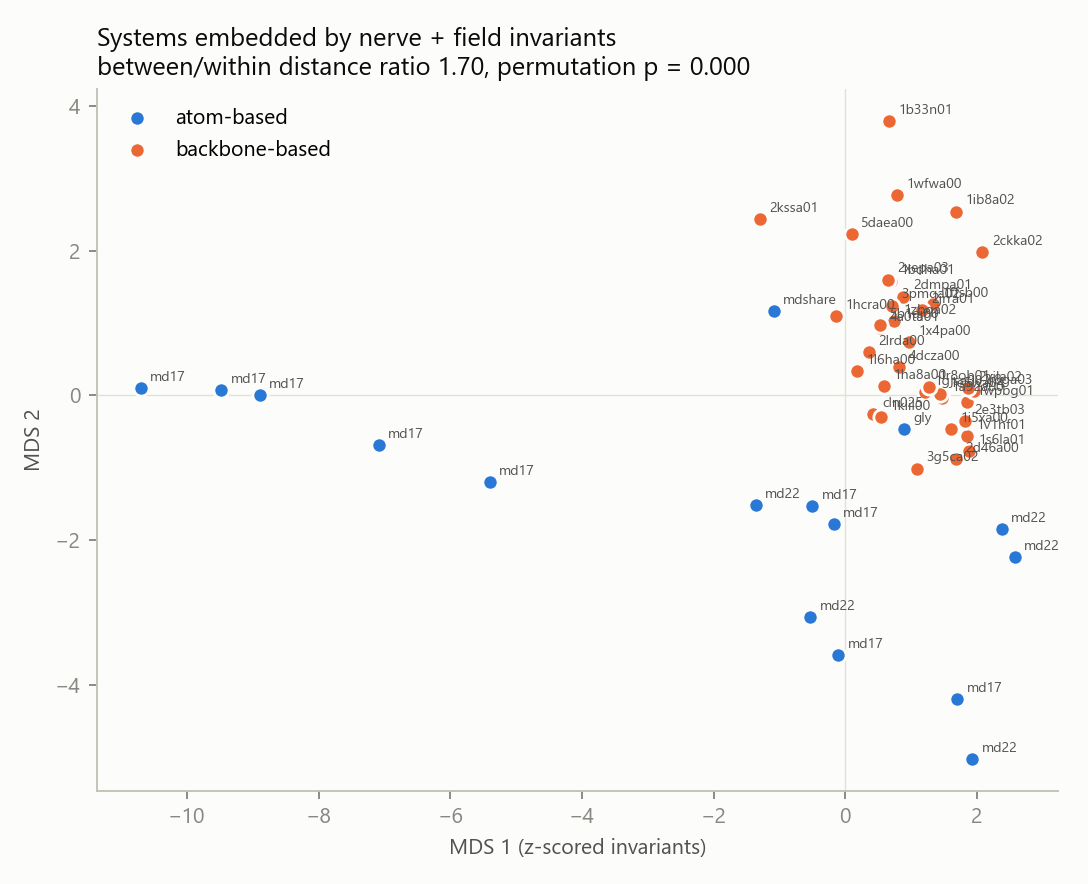
\includegraphics[width=.72\linewidth]{figures/fig_embedding.png}
\caption{Systems embedded by nerve and deformation-field invariants. Blue: atom-based; orange: backbone-based.}\label{fig:embedding}\end{figure}
\begin{figure}[H]\centering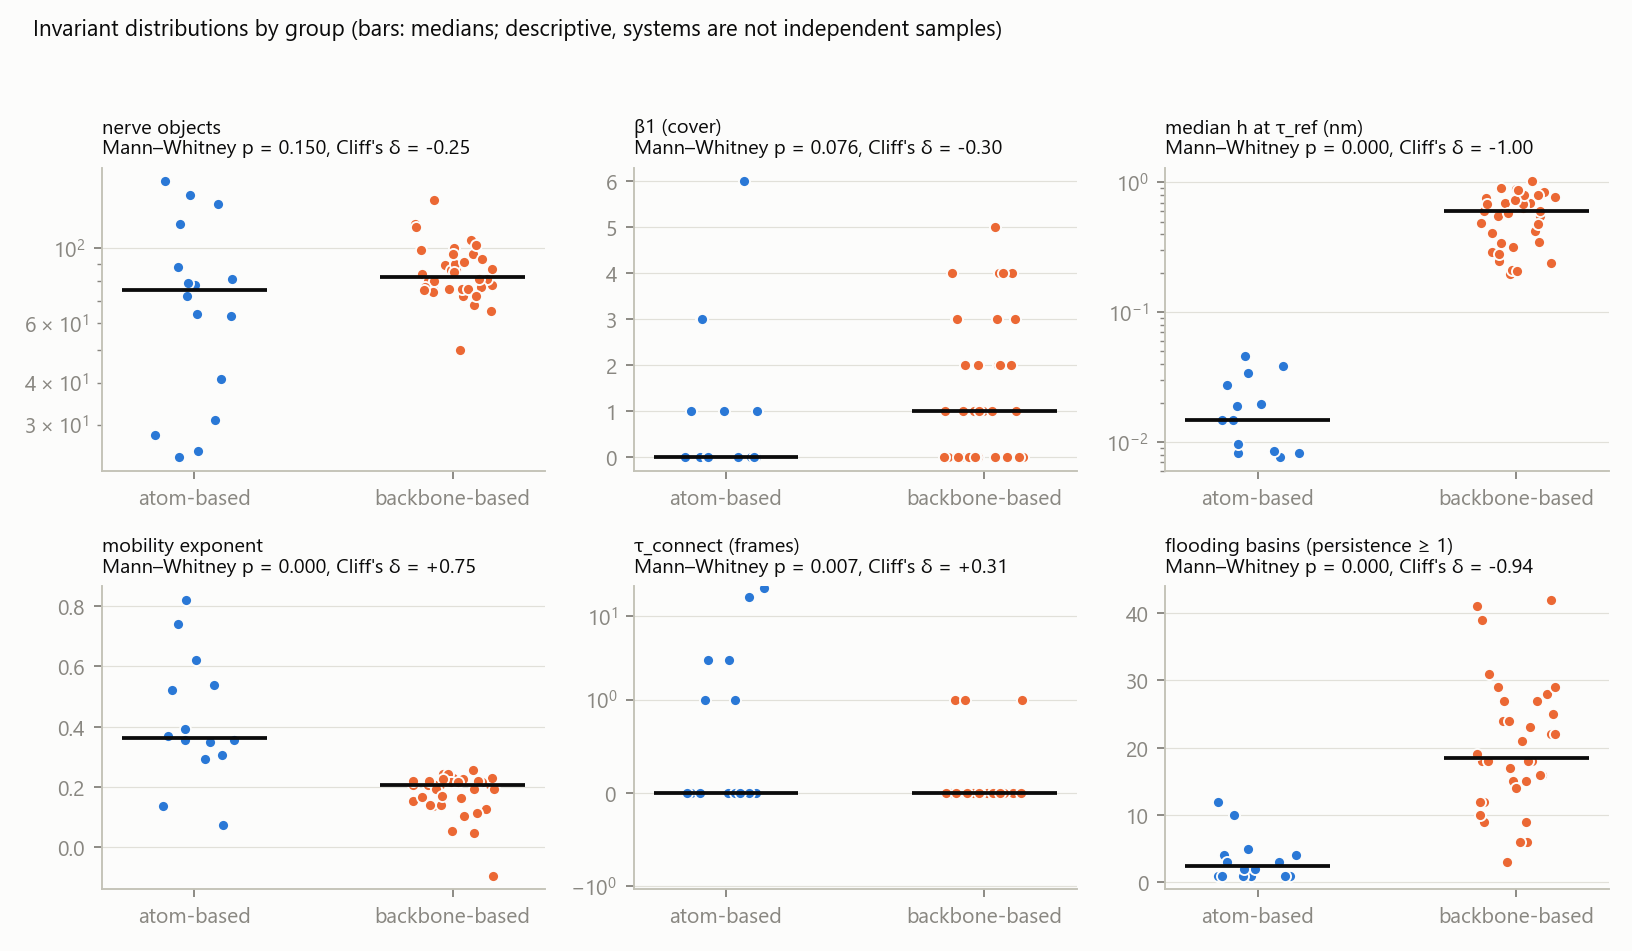
\includegraphics[width=\linewidth]{figures/fig_invariants.png}
\caption{Invariant distributions by group. Bars mark medians; tests are descriptive because systems are not independent samples (the dipeptide family shares a protocol, the mdCATH domains share a dataset).}\label{fig:invariants}\end{figure}
\begin{figure}[H]\centering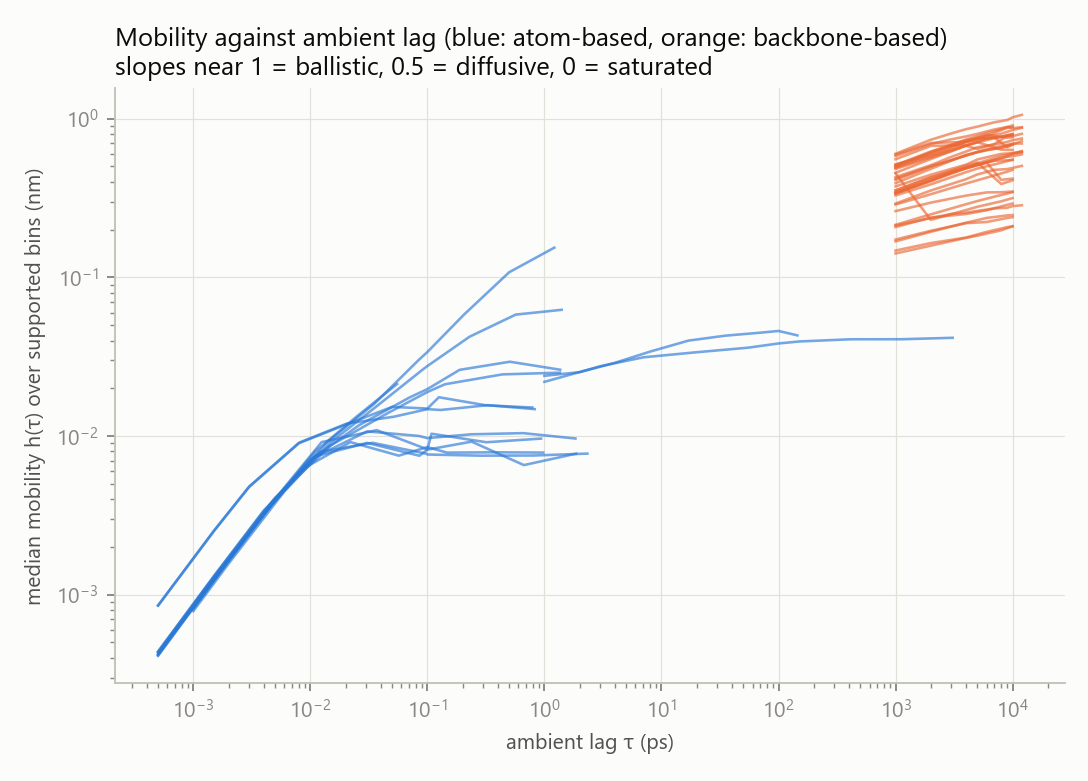
\includegraphics[width=.72\linewidth]{figures/fig_scaling.png}
\caption{Median mobility against ambient lag. Ab initio trajectories sampled every femtosecond show the ballistic regime; picosecond- and nanosecond-sampled systems are saturated.}\label{fig:scaling}\end{figure}
\begin{figure}[H]\centering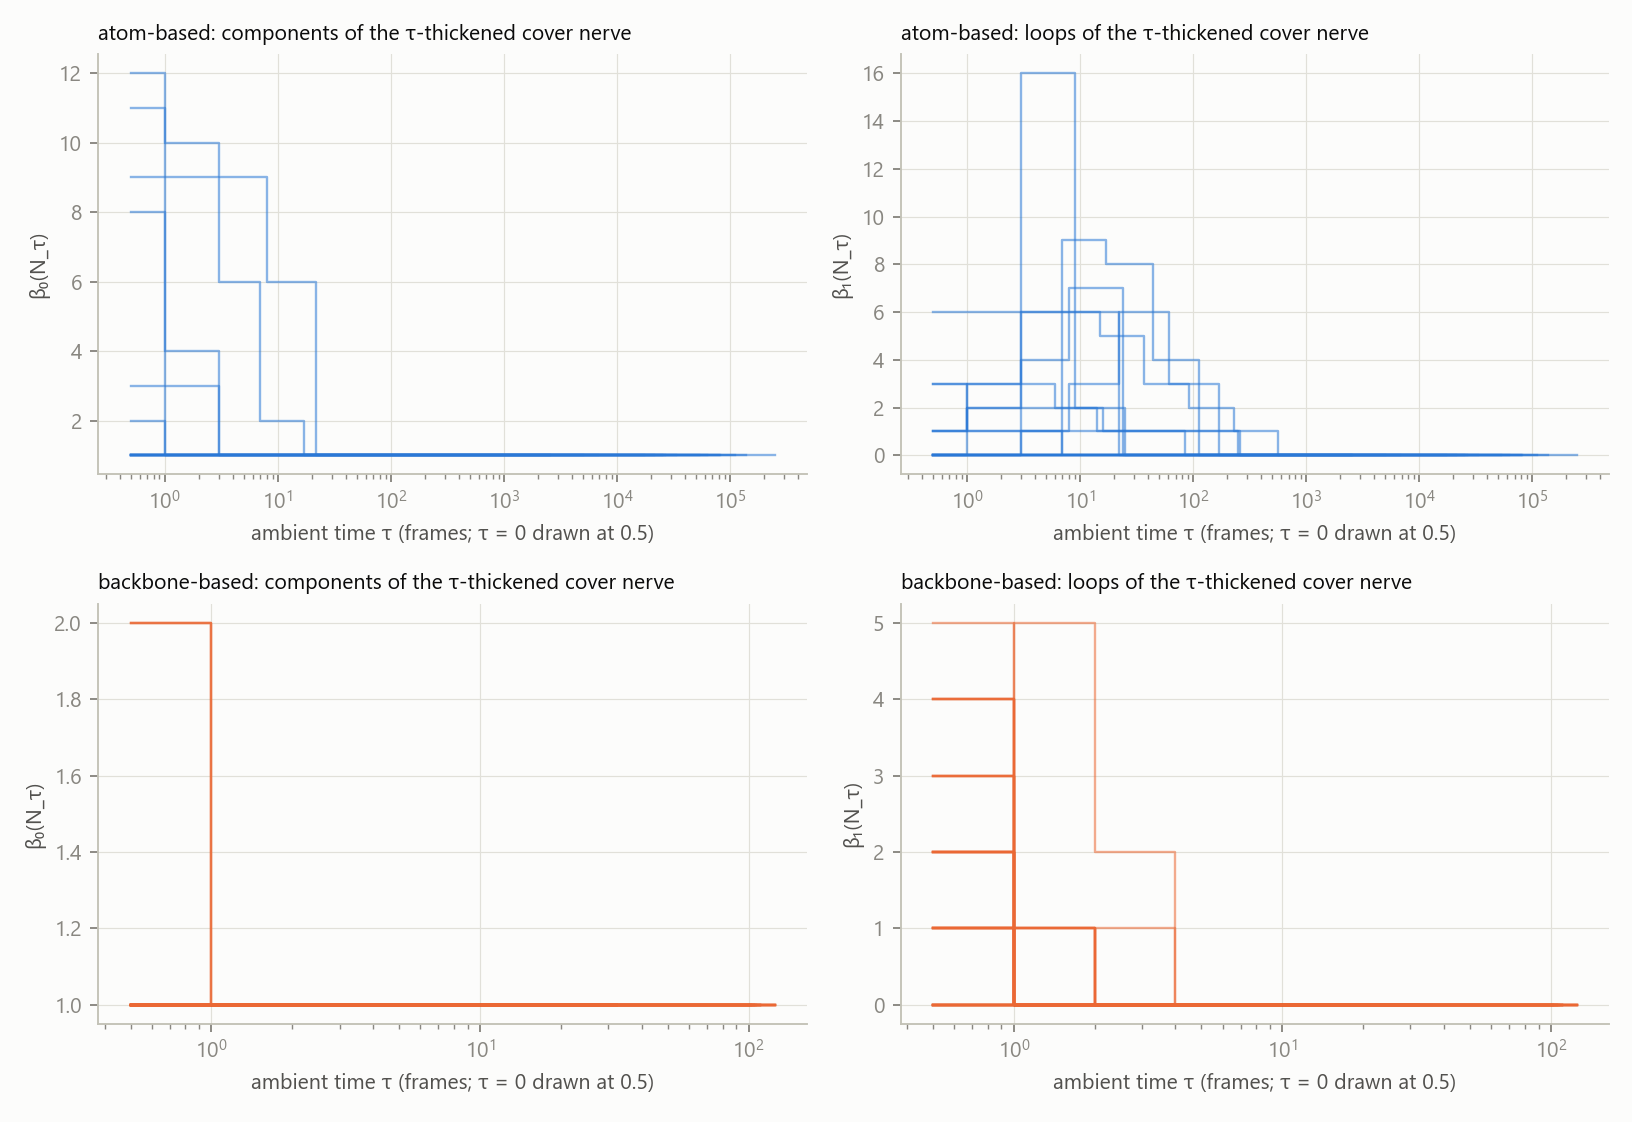
\includegraphics[width=\linewidth]{figures/fig_betti_curves.png}
\caption{Fluid filtration: $\beta_0(N_\tau)/\beta_0(N_0)$ against $\tau/\tau_{\mathrm c}$.}\label{fig:betti}\end{figure}

\subsection{Rigidity test}
Theorem~\ref{thm:rigid} predicts that cover membership is invariant between frames that are first-order close relative to the cover. We measure the \emph{membership flip rate}: the fraction of consecutive within-run frame pairs whose 18-ball membership vector differs. Classifying by the early mobility exponent $\alpha_{\mathrm{early}}$ (log--log slope over the first half of the lag ladder), 12 of the 69 primary systems are ballistic ($\alpha_{\mathrm{early}}>0.6$) and 32 are saturated ($\alpha_{\mathrm{early}}<0.2$). The mean one-frame flip rate is 0.023 for the ballistic systems and 0.790 for the saturated ones (Spearman $\rho=-0.82$, $p=0.000$, $n=69$ between the early exponent and the flip rate). The relative drop of $\beta_0$ between $\tau=0$ and the first ladder lag is 0.15 (ballistic) against 0.08 (saturated); this statistic is dominated by isolated fringe balls, which a single frame of thickening attaches to the main component, so the flip rate is the cleaner test. Ballistic systems: sgdml-md17-aspirin, sgdml-md17-azobenzene, sgdml-md17-ethanol, sgdml-md17-malonaldehyde, sgdml-md17-naphthalene, sgdml-md17-paracetamol, sgdml-md17-salicylic, sgdml-md17-toluene, sgdml-md17-uracil, sgdml-md22-ac-ala3-nhme, sgdml-md22-dha, sgdml-md22-stachyose.


\subsection{Comparison between atomistic and C$\alpha$ state categories}\label{sec:functor}
For each mdCATH domain the heavy-atom and C$\alpha$ covers are built on identical frames. Mapping every heavy-atom face $\sigma$ to the C$\alpha$ face with the largest witness-set Jaccard index, $f(\sigma)$, we ask whether strict inclusions and composable pairs are preserved (laxly, allowing equal images). Table~\ref{tab:functor} and Figure~\ref{fig:functor} report the rates. A rate of one in both directions would make $f$ a functor between the face posets; the measured shortfall quantifies the approximation error asked for in the atlas's sixth research question.

\begin{table}[H]\centering\small\begin{tabular}{lrrrrrr}\toprule
domain & faces (heavy/C$\alpha$) & med.\ Jaccard & incl.\ lax & incl.\ strict & comp.\ lax & C$\alpha\to$heavy incl.\\\midrule
1a92a00 & 110/91 & 0.17 & 0.62 & 0.36 & 0.42 & 0.69\\
1b33n01 & 69/83 & 0.10 & 0.44 & 0.25 & 0.16 & 0.48\\
1bdha01 & 77/76 & 0.28 & 0.75 & 0.54 & 0.59 & 0.72\\
1e5wa04 & 101/102 & 0.28 & 0.63 & 0.42 & 0.46 & 0.69\\
1ffsb00 & 158/176 & 0.21 & 0.53 & 0.36 & 0.31 & 0.63\\
1gjsa00 & 106/90 & 0.26 & 0.72 & 0.48 & 0.54 & 0.60\\
1ha8a00 & 80/80 & 0.20 & 0.59 & 0.37 & 0.33 & 0.59\\
1hcra00 & 77/65 & 0.21 & 0.74 & 0.51 & 0.64 & 0.64\\
1i5xa00 & 102/115 & 0.28 & 0.67 & 0.53 & 0.43 & 0.81\\
1ib8a02 & 106/91 & 0.15 & 0.64 & 0.42 & 0.45 & 0.49\\
1klil00 & 80/82 & 0.17 & 0.64 & 0.39 & 0.44 & 0.64\\
1l6ha00 & 100/77 & 0.21 & 0.70 & 0.45 & 0.52 & 0.67\\
1r8ob01 & 86/90 & 0.30 & 0.73 & 0.58 & 0.56 & 0.69\\
1s6la01 & 134/107 & 0.26 & 0.62 & 0.43 & 0.40 & 0.72\\
1v1hf01 & 94/107 & 0.30 & 0.72 & 0.54 & 0.58 & 0.66\\
1wfwa00 & 82/73 & 0.28 & 0.72 & 0.51 & 0.57 & 0.74\\
1wpbg01 & 112/112 & 0.27 & 0.73 & 0.51 & 0.53 & 0.62\\
1x4pa00 & 78/77 & 0.20 & 0.66 & 0.44 & 0.41 & 0.67\\
1zbqa02 & 65/84 & 0.21 & 0.72 & 0.49 & 0.54 & 0.69\\
2ckka02 & 181/134 & 0.14 & 0.63 & 0.40 & 0.46 & 0.56\\
2d46a00 & 95/93 & 0.29 & 0.56 & 0.37 & 0.30 & 0.66\\
2dmpa01 & 99/77 & 0.26 & 0.69 & 0.49 & 0.48 & 0.75\\
2e3tb03 & 181/129 & 0.23 & 0.57 & 0.36 & 0.34 & 0.62\\
2j8ga03 & 72/95 & 0.30 & 0.71 & 0.47 & 0.57 & 0.68\\
2jrra01 & 142/101 & 0.25 & 0.65 & 0.46 & 0.45 & 0.70\\
2kssa01 & 64/50 & 0.20 & 0.69 & 0.39 & 0.48 & 0.68\\
2lrda00 & 116/75 & 0.22 & 0.68 & 0.47 & 0.48 & 0.65\\
2xepa03 & 88/79 & 0.11 & 0.56 & 0.39 & 0.36 & 0.68\\
2yila02 & 75/109 & 0.23 & 0.64 & 0.44 & 0.37 & 0.72\\
3g5ca02 & 79/87 & 0.30 & 0.72 & 0.56 & 0.48 & 0.79\\
3pmqa02 & 73/69 & 0.21 & 0.76 & 0.46 & 0.64 & 0.70\\
4a0ta01 & 96/76 & 0.37 & 0.72 & 0.56 & 0.50 & 0.79\\
4dcza00 & 87/82 & 0.25 & 0.64 & 0.43 & 0.43 & 0.70\\
5b1aj00 & 90/78 & 0.07 & 0.48 & 0.29 & 0.25 & 0.50\\
5daea00 & 83/72 & 0.28 & 0.77 & 0.48 & 0.65 & 0.70\\
\midrule
median over domains & & 0.23 & 0.67 & 0.45 & 0.46 & 0.68\\
\bottomrule\end{tabular}\caption{Comparison of face posets built from heavy atoms and from C$\alpha$ sites on identical frames (mdCATH).}\label{tab:functor}\end{table}

\begin{figure}[H]\centering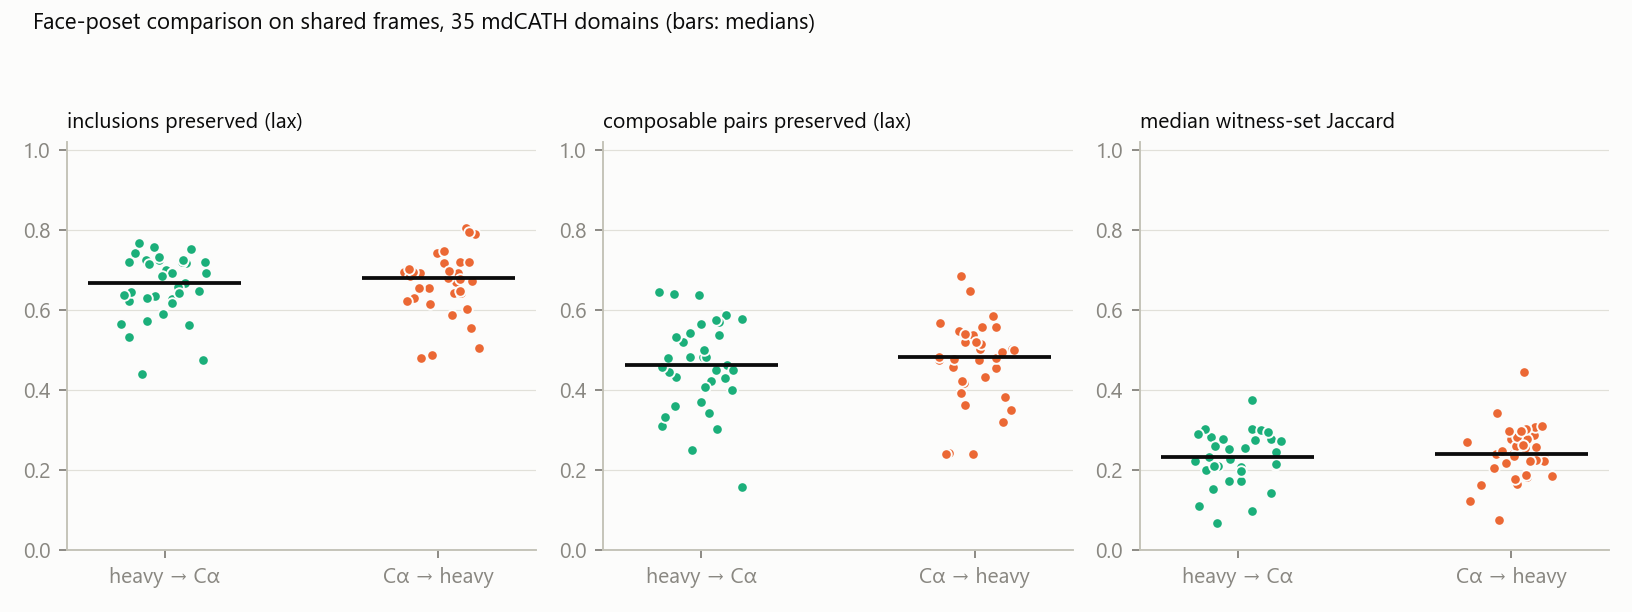
\includegraphics[width=.9\linewidth]{figures/fig_functor.png}
\caption{Face-poset comparison between the heavy-atom and C$\alpha$ representations of each mdCATH domain, in both directions.}\label{fig:functor}\end{figure}

\subsection{Temperature ladder}
\begin{table}[H]\centering\small\begin{tabular}{lrrrrr}\toprule temperature (K) & 320 & 348 & 379 & 413 & 450\\\midrule
median $\beta_0$ & 1.0 & 1.0 & 1.0 & 1.0 & 1.0\\
median triangles & 12 & 16 & 19 & 20 & 23\\
median $h$ at $\tau_{\mathrm{ref}}$ (nm) & 0.232 & 0.287 & 0.372 & 0.578 & 0.861\\
\bottomrule\end{tabular}\caption{mdCATH temperature ladder over 35 domains (same chart and cover per domain).}\label{tab:temperature}\end{table}

\begin{figure}[H]\centering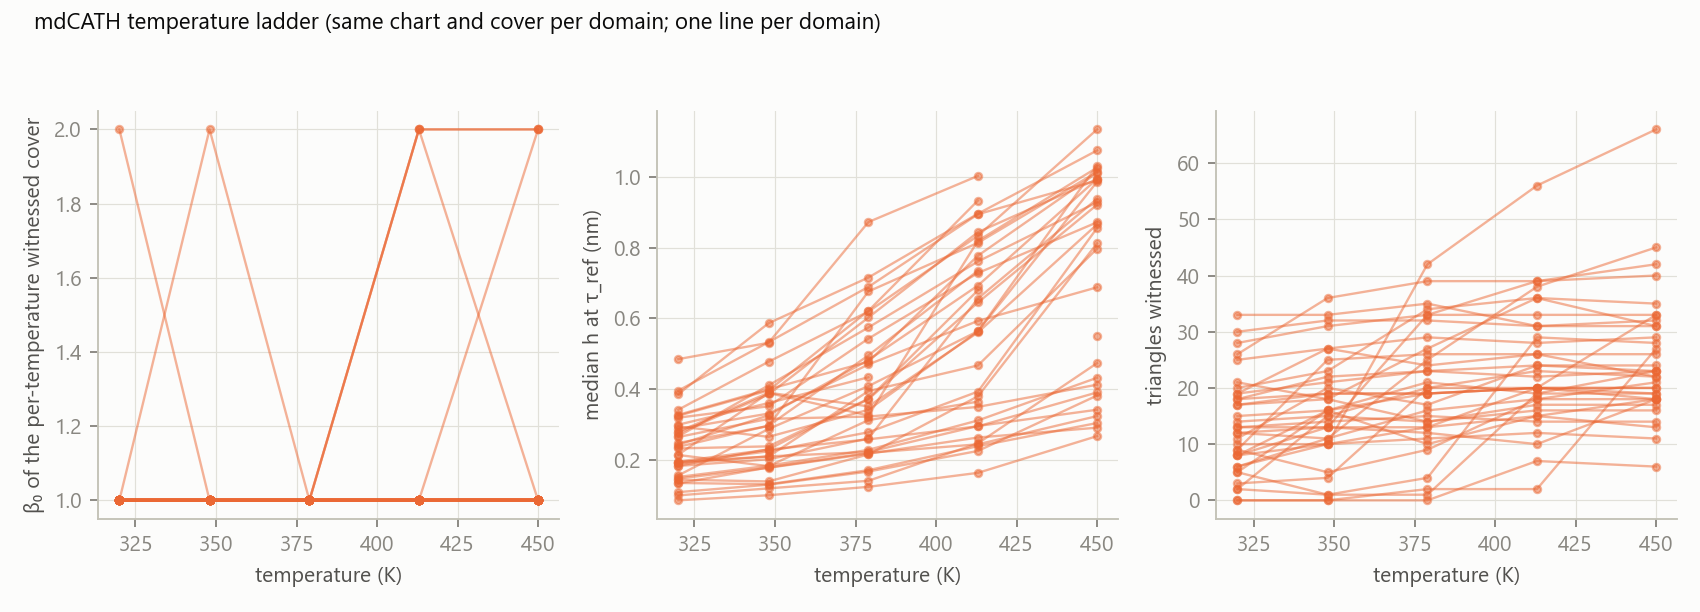
\includegraphics[width=\linewidth]{figures/fig_temperature.png}
\caption{mdCATH temperature ladder: per-temperature witnessed cover and field in the shared chart and cover of each domain.}\label{fig:temperature}\end{figure}

\subsection{Exemplars}
\begin{figure}[H]\centering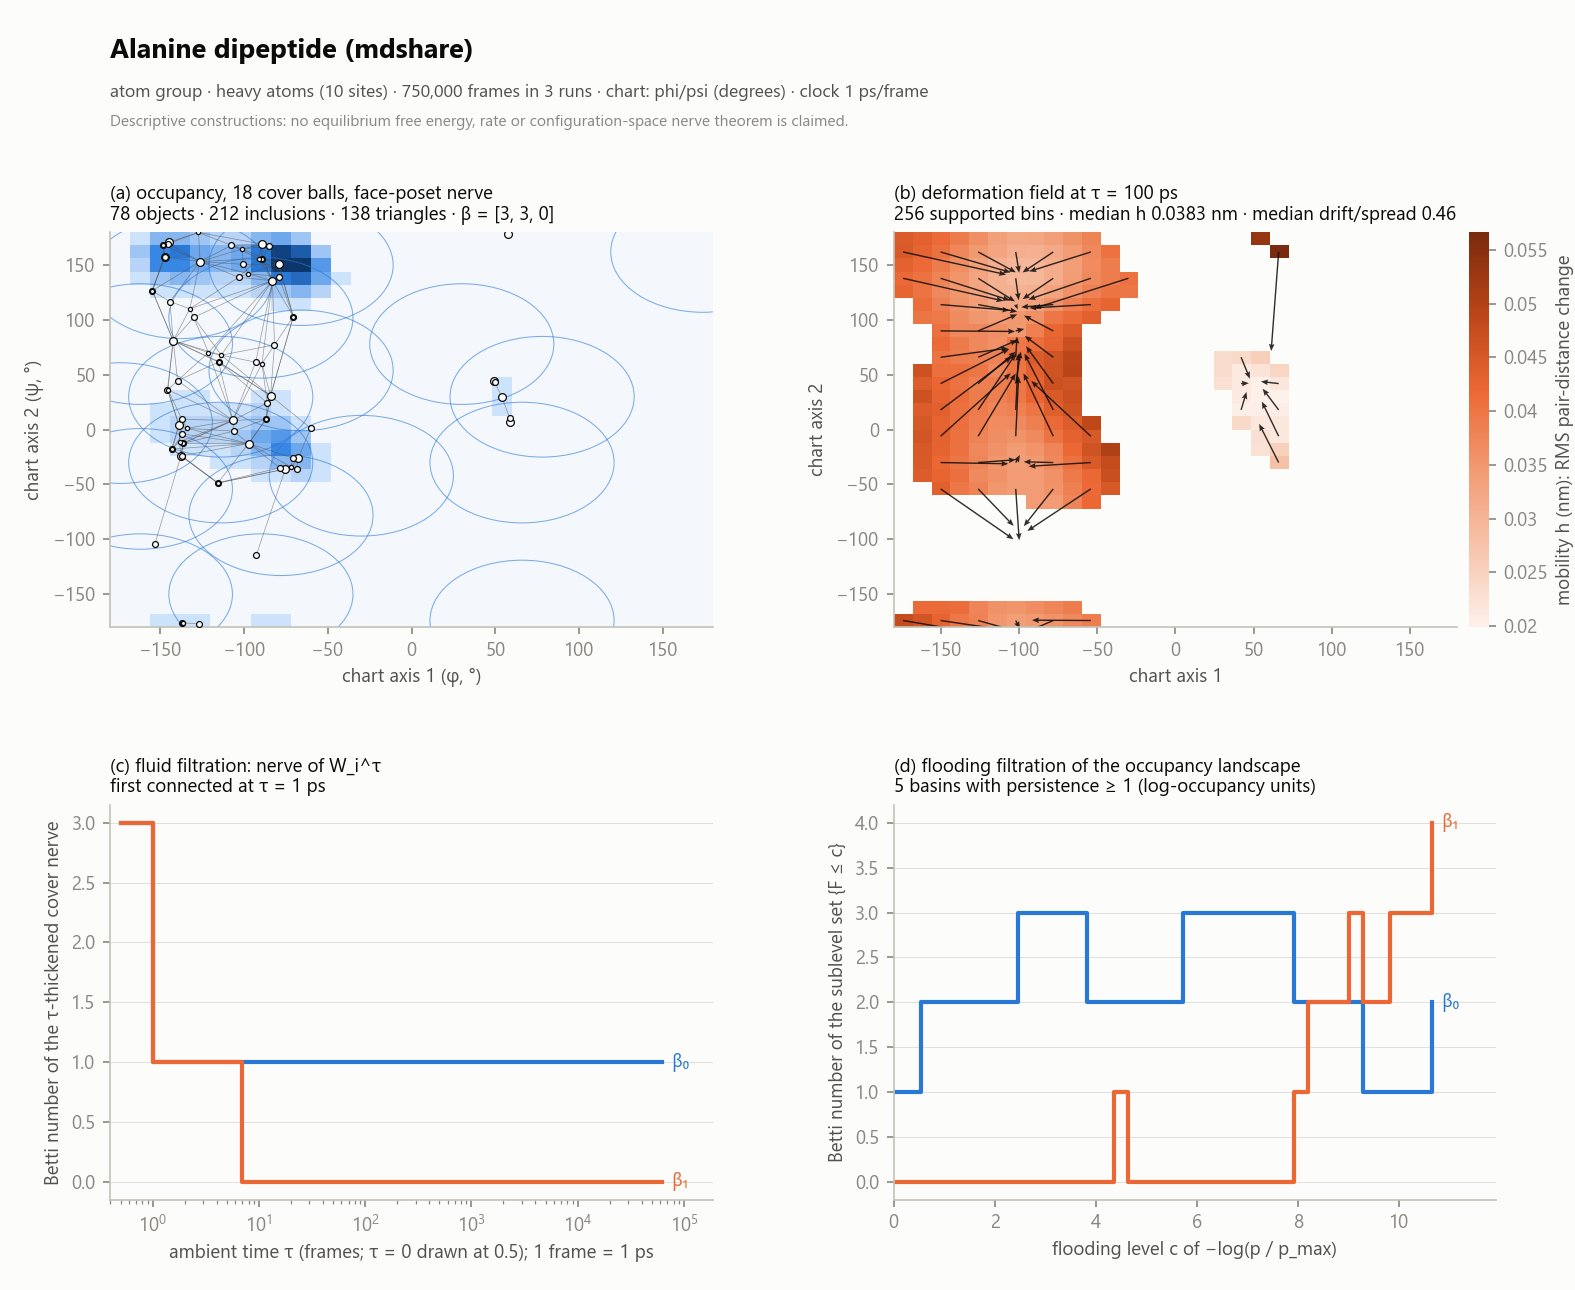
\includegraphics[width=\linewidth]{figures/system_ala2.png}\caption{Alanine dipeptide (mdshare): occupancy and nerve, deformation field, fluid and flooding filtrations.}\end{figure}
\begin{figure}[H]\centering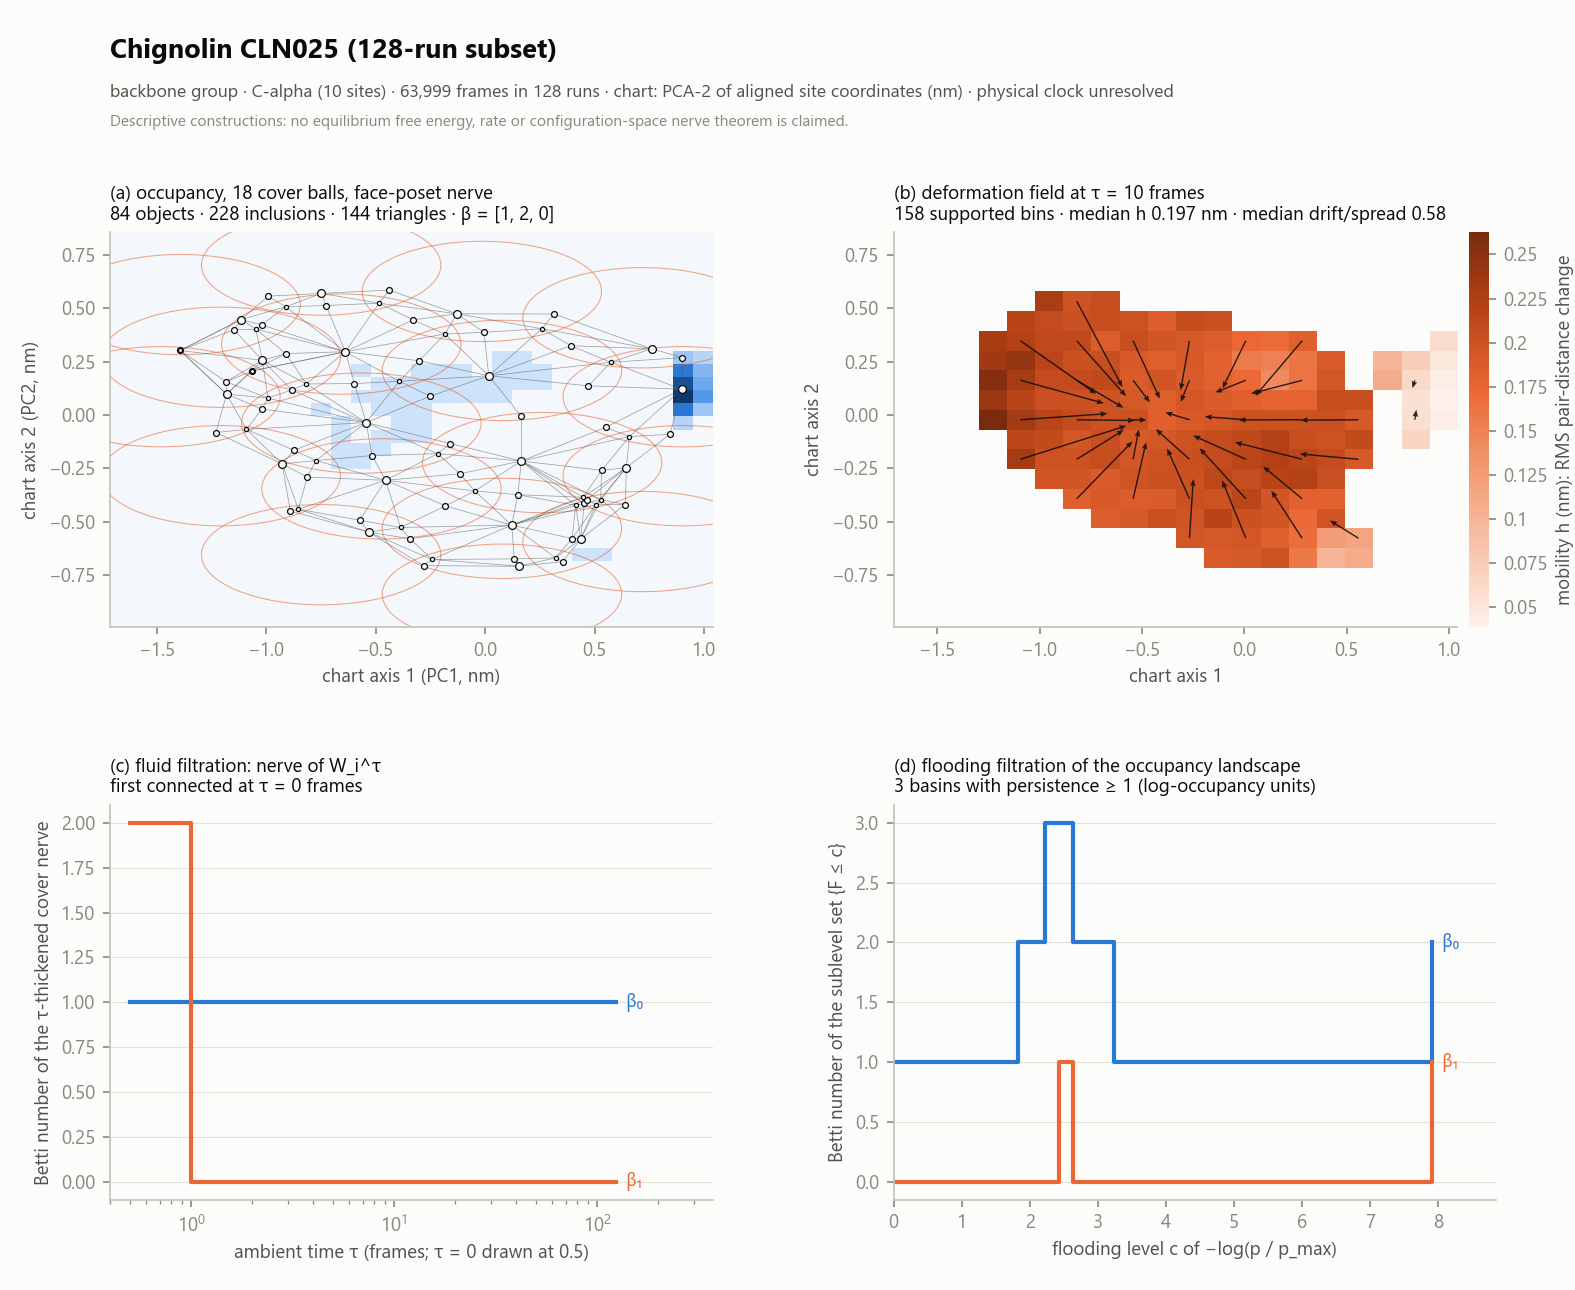
\includegraphics[width=\linewidth]{figures/system_cln025.png}\caption{Chignolin CLN025 (128-run subset): occupancy and nerve, deformation field, fluid and flooding filtrations.}\end{figure}
\begin{figure}[H]\centering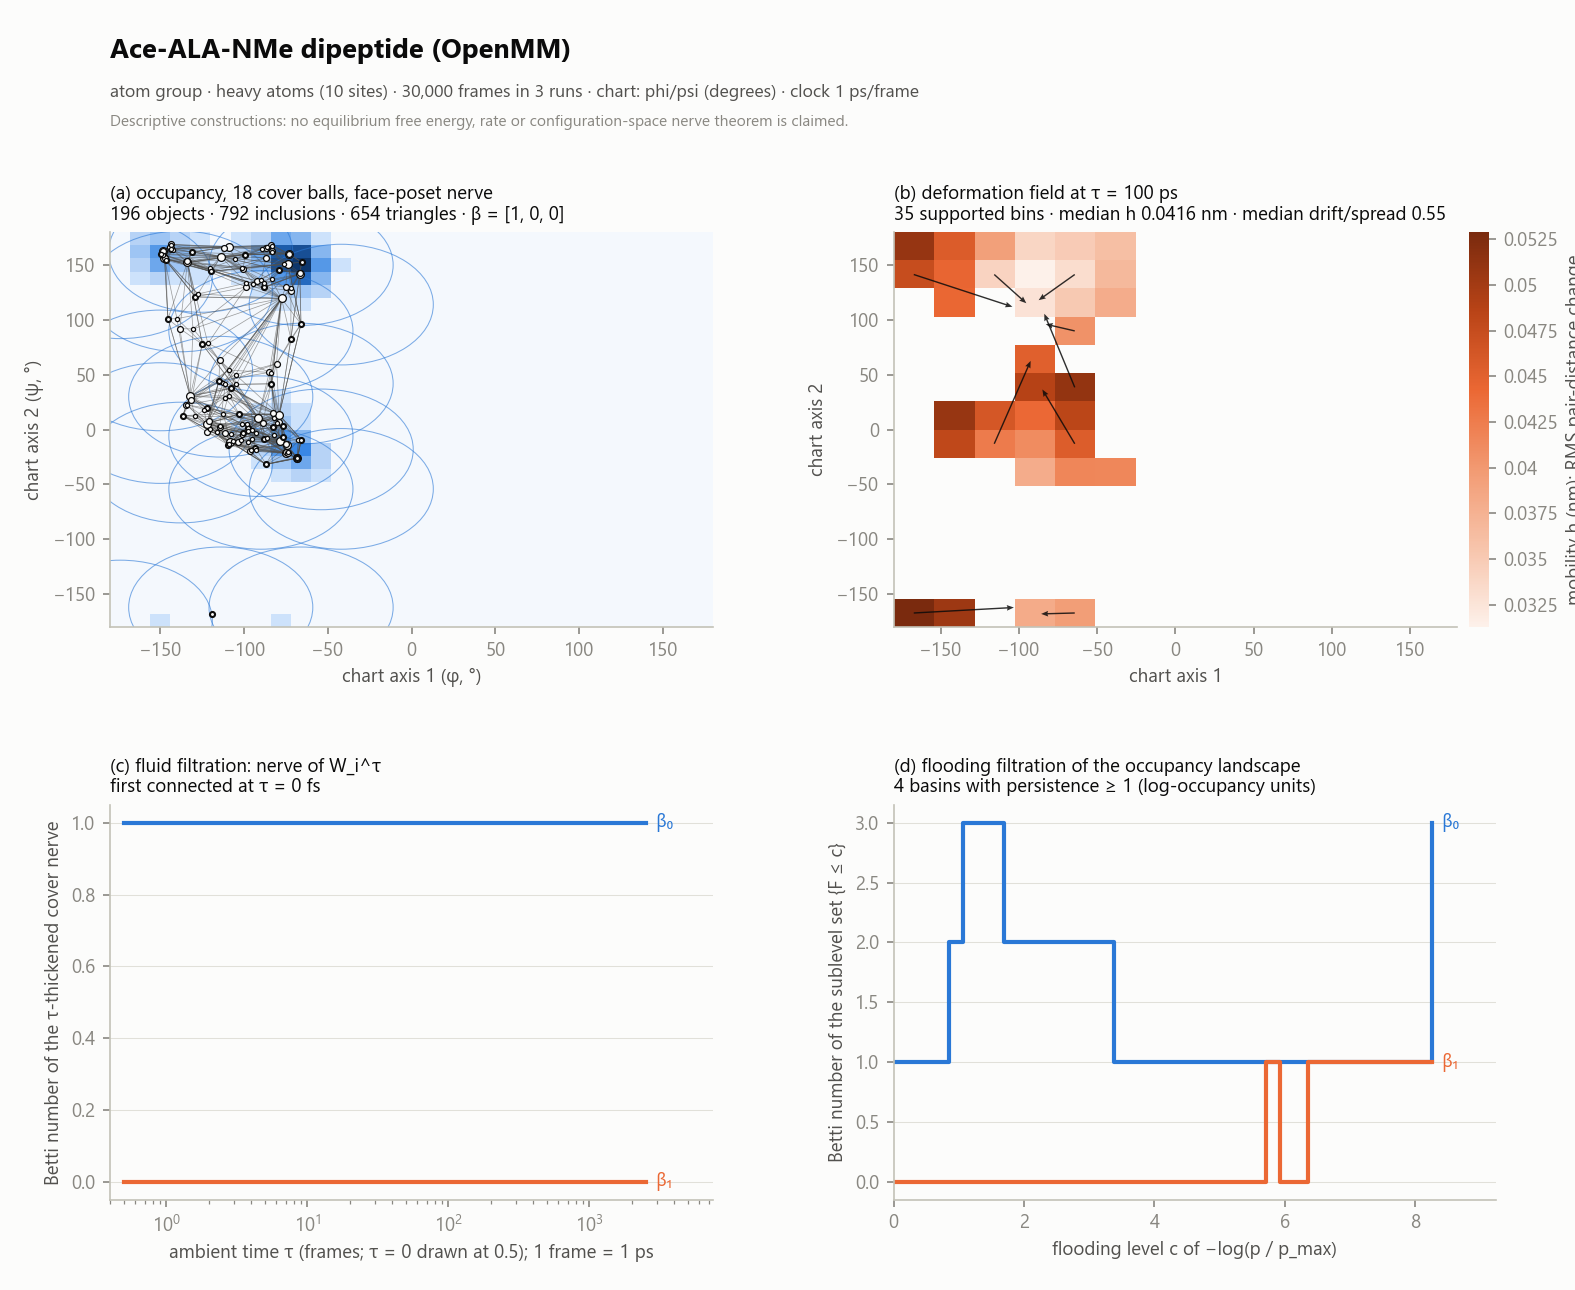
\includegraphics[width=\linewidth]{figures/system_dipeptide-ala.png}\caption{Ace-ALA-NMe dipeptide (OpenMM): occupancy and nerve, deformation field, fluid and flooding filtrations.}\end{figure}
\begin{figure}[H]\centering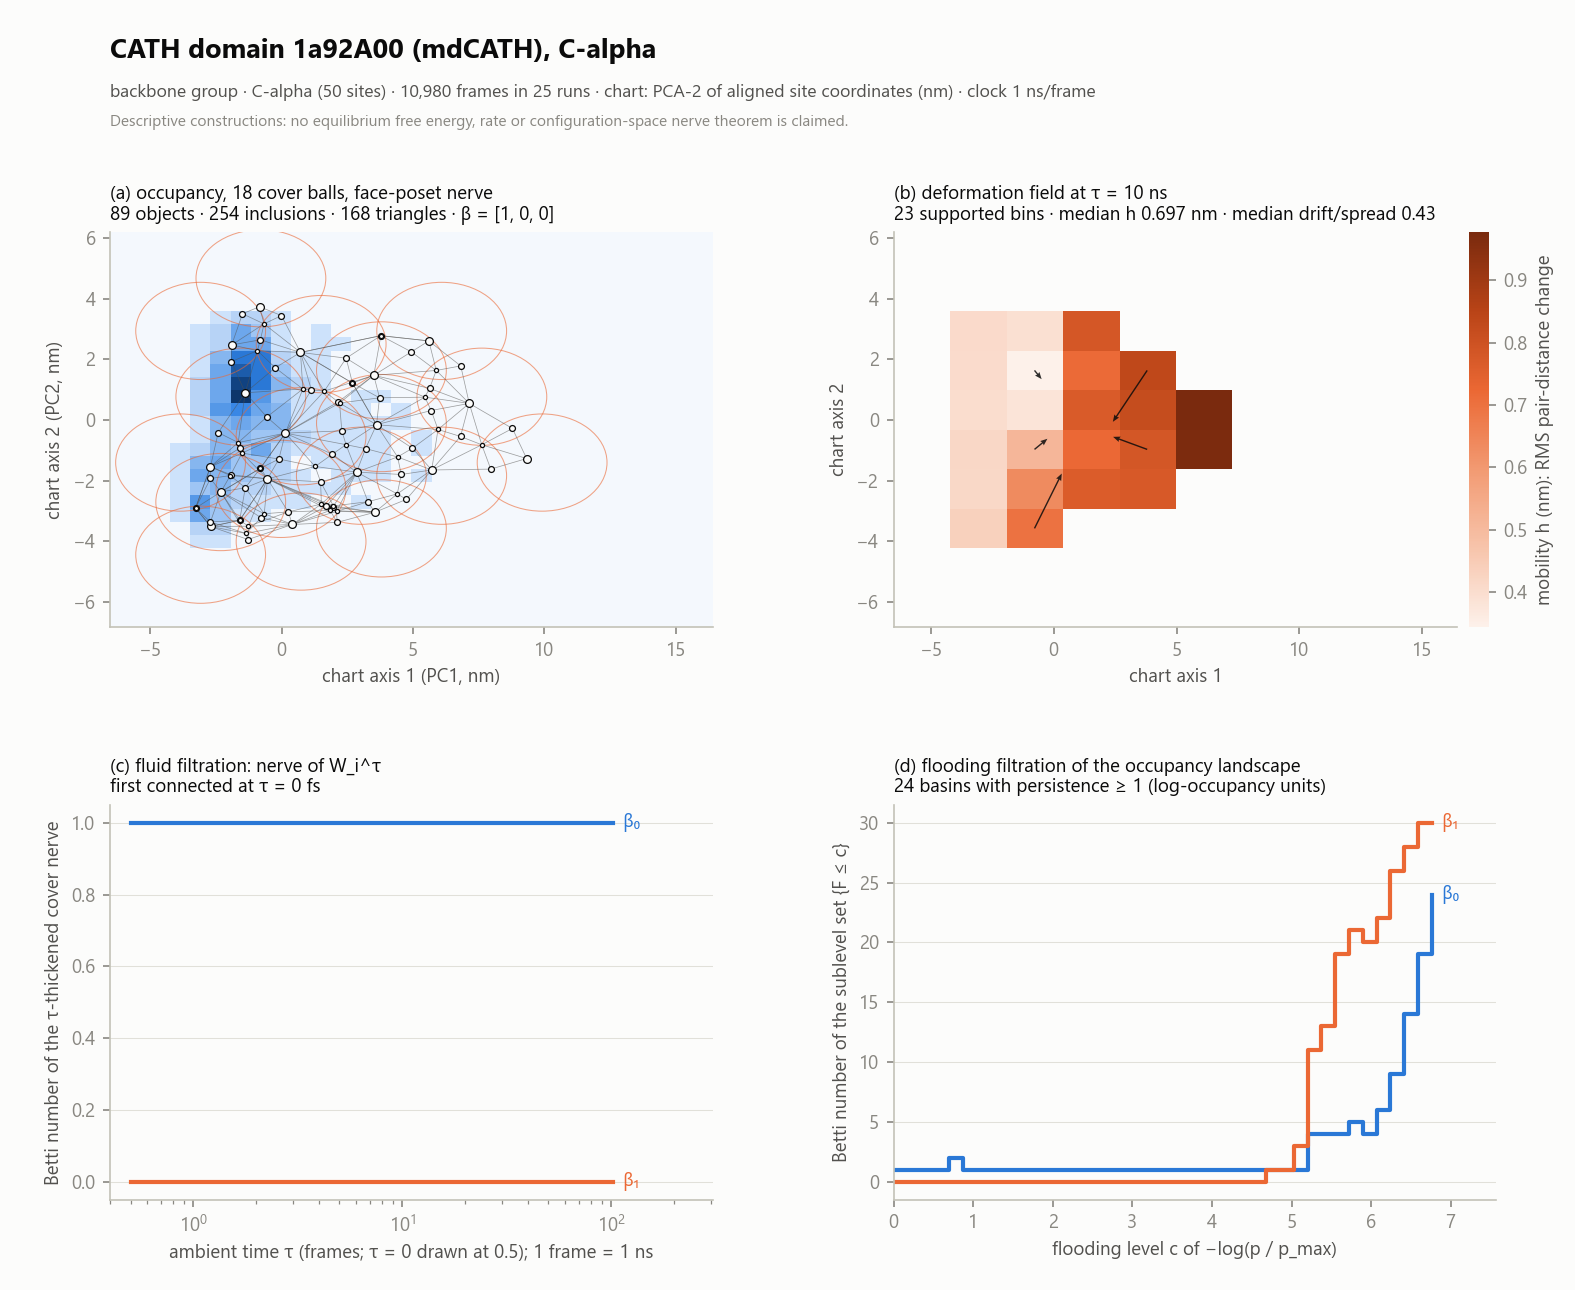
\includegraphics[width=\linewidth]{figures/system_mdcath-1a92a00-ca.png}\caption{CATH domain 1a92A00 (mdCATH), C-alpha: occupancy and nerve, deformation field, fluid and flooding filtrations.}\end{figure}
\begin{figure}[H]\centering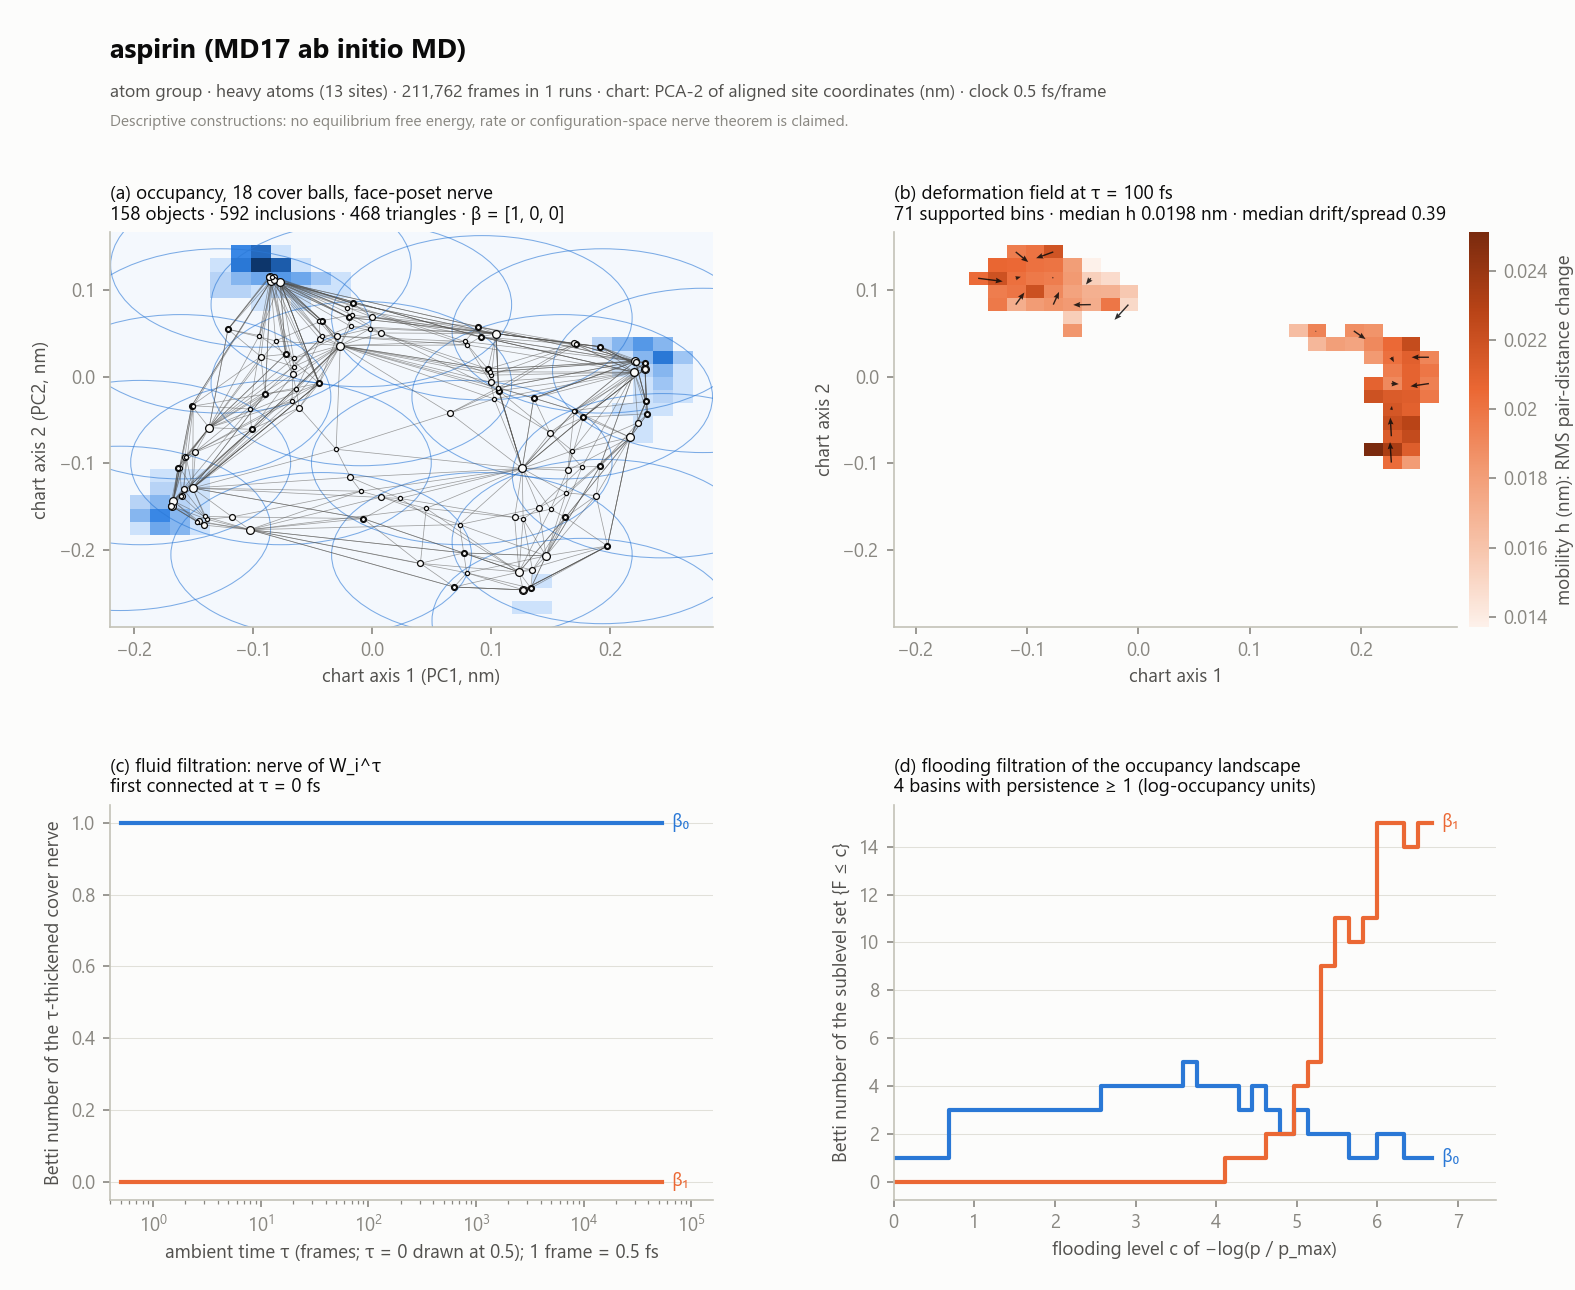
\includegraphics[width=\linewidth]{figures/system_sgdml-md17-aspirin.png}\caption{aspirin (MD17 ab initio MD): occupancy and nerve, deformation field, fluid and flooding filtrations.}\end{figure}
\begin{figure}[H]\centering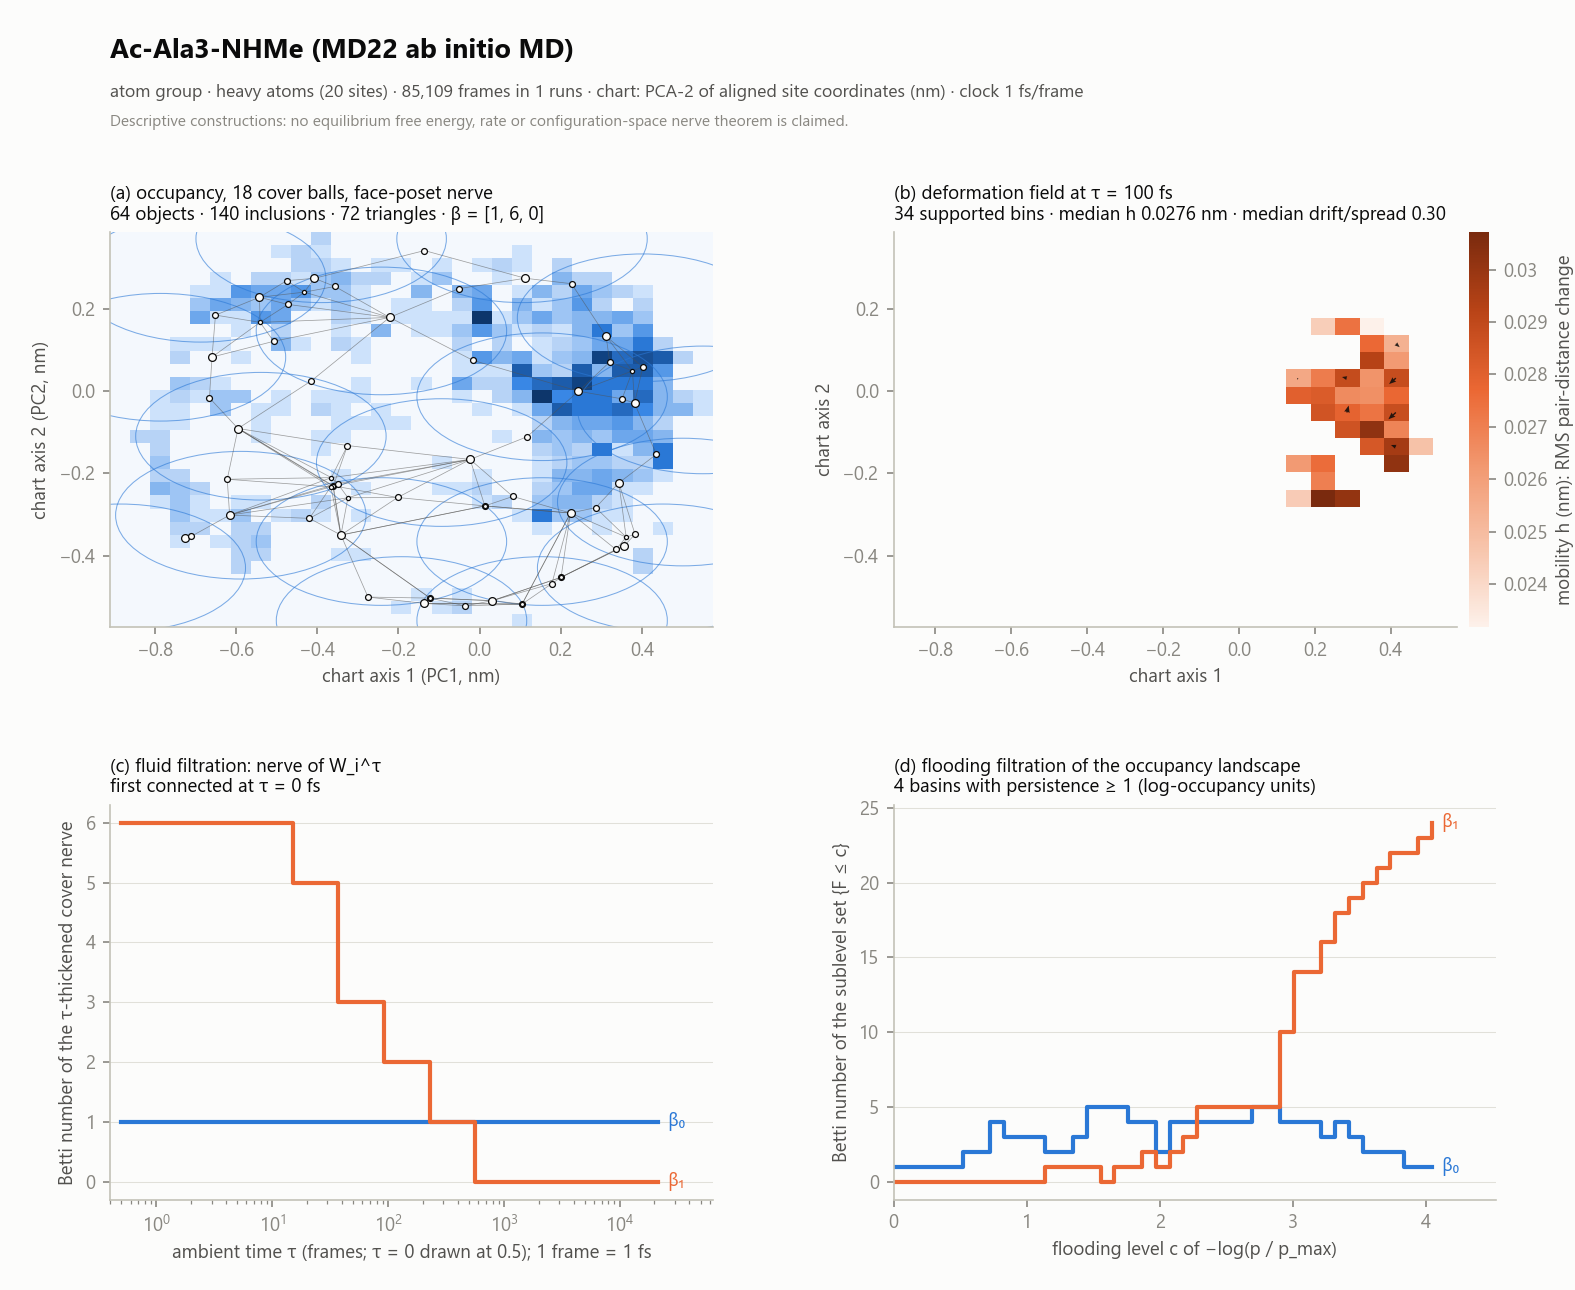
\includegraphics[width=\linewidth]{figures/system_sgdml-md22-ac-ala3-nhme.png}\caption{Ac-Ala3-NHMe (MD22 ab initio MD): occupancy and nerve, deformation field, fluid and flooding filtrations.}\end{figure}


\section{Limitations}
Charts are two-dimensional projections (PCA or two dihedrals); the fibre over a chart bin is averaged, and nothing about the full configuration space is asserted. Covers use a single declared radius with a sensitivity ladder, not an optimised scale. Homology is over GF(2). The MD17/MD22 systems are single ab initio trajectories at elevated temperature with nominal time steps taken from the dataset papers; the dipeptide family comes from short new implicit-solvent simulations; mdCATH frames are 1\,ns apart, which makes every per-frame quantity saturated; CLN025 has no physical clock. Support thresholds leave bins empty rather than filling them; three single-trajectory MD22 systems (AT-AT, AT-AT-CG-CG, stachyose) revisit chart bins in fewer than five blocks and therefore have no supported mobility at the reference lag. The comparison functor is an empirical best-match map, not a proved functor. The SDG results concern an idealisation (formally open covers, smooth flows) and are used to interpret, not to validate, the measurements. The flooding filtration is a geometric analogue of metadynamics computed from occupancy; no biased simulation was run. None of the constructions is a kinetic model, and the pooled occupancy is not an equilibrium free energy.

\section{Reproduction}
From \texttt{fluid-nerve/}: \texttt{python acquire\_sgdml.py}, \texttt{python acquire\_mdcath.py}, \texttt{python generate\_dipeptides.py}, \texttt{python build\_all.py}, \texttt{python render.py}, \texttt{python export\_homotopy.py}, \texttt{python compare\_all.py}, \texttt{python theory/make\_results.py}, \texttt{tectonic theory/fluid-nerve-theory.tex}. Unit tests on synthetic data: \texttt{python -m unittest discover -s tests}. Raw data are not committed; manifests with SHA-256 hashes are.

\begin{thebibliography}{9}
\bibitem{kock2006} A.~Kock, \emph{Synthetic Differential Geometry}, 2nd ed., LMS Lecture Note Series 333, Cambridge University Press, 2006.
\bibitem{kock2010} A.~Kock, \emph{Synthetic Geometry of Manifolds}, Cambridge Tracts in Mathematics 180, Cambridge University Press, 2010.
\bibitem{lavendhomme} R.~Lavendhomme, \emph{Basic Concepts of Synthetic Differential Geometry}, Kluwer, 1996.
\bibitem{penon} J.~Penon, Infinit\'esimaux et intuitionnisme, \emph{Cahiers Topologie G\'eom.\ Diff\'erentielle} 22 (1981) 67--72.
\bibitem{street} R.~Street, The algebra of oriented simplexes, \emph{J.\ Pure Appl.\ Algebra} 49 (1987) 283--335.
\bibitem{homotopyio} N.~Corbyn, L.~Heidemann, N.~Hu, C.~Sarti, C.~Tataru, J.~Vicary, homotopy.io: a proof assistant for finitely-presented globular $n$-categories, FSCD 2024; arXiv:2402.13179.
\bibitem{mdcath} A.~Mirarchi, T.~Giorgino, G.~De Fabritiis, mdCATH: a large-scale MD dataset for data-driven computational biophysics, \emph{Sci.\ Data} 11 (2024) 1299.
\bibitem{md17} S.~Chmiela et al., Machine learning of accurate energy-conserving molecular force fields, \emph{Sci.\ Adv.} 3 (2017) e1603015; S.~Chmiela et al., Accurate global machine learning force fields for molecules with hundreds of atoms, \emph{Sci.\ Adv.} 9 (2023) eadf0873.
\bibitem{cln} A.~P\'erez Culubret, G.~De Fabritiis, Chignolin simulations, figshare (2021), doi:10.6084/m9.figshare.13858898.
\bibitem{metad} A.~Laio, M.~Parrinello, Escaping free-energy minima, \emph{PNAS} 99 (2002) 12562--12566.
\end{thebibliography}
\end{document}
